\documentclass[11pt, a4paper, twocolumn]{article}

\title{\textbf{A SSD study for Object Detection in Open Images Dataset v5}}
\author{Bruno de Almeida Silveira}
\date{January 2020}

\usepackage{url}
\usepackage{hyperref}
\usepackage{indentfirst}

\usepackage{booktabs}
\usepackage[table,xcdraw]{xcolor}

\usepackage{adjustbox}
\usepackage{lipsum}
\usepackage{caption}

\usepackage{amsmath}

\usepackage{graphicx}

\usepackage{xurl}

\usepackage{titling}
\usepackage{blindtext}

\usepackage{subfig}

\usepackage{appendix}
\usepackage{etoolbox}
\BeforeBeginEnvironment{appendices}{\clearpage}

\graphicspath{ {./images/} }
\begin{document}

\begin{titlingpage}
	\maketitle
	\begin{abstract}
		This project is a study in the computer vision field, more specifically, the object detection area. The project presents a study in a very disseminated solution called Single Shot Detection, which designed a solution using a deep neural network that intends to classify and find as many bounding boxes it can on an image. The central concept of this approach is the performance of the model, making it possible to be used in many different solutions, delivering a more feasible result. This project also proposes some simple changes using different architectures plugged in the SSD design, such as, MobileNet, ResNet and Xception.
	\end{abstract}
\end{titlingpage}

\section{Definition}
\subsection{Project Overview}
The main challenge in this project is to create a model that identifies objects in images. This challenge involves two main tasks. The former is to identify object positions in a picture, and the latter is to classify those objects correctly. 

\begin{figure}[ht]
	\centering
	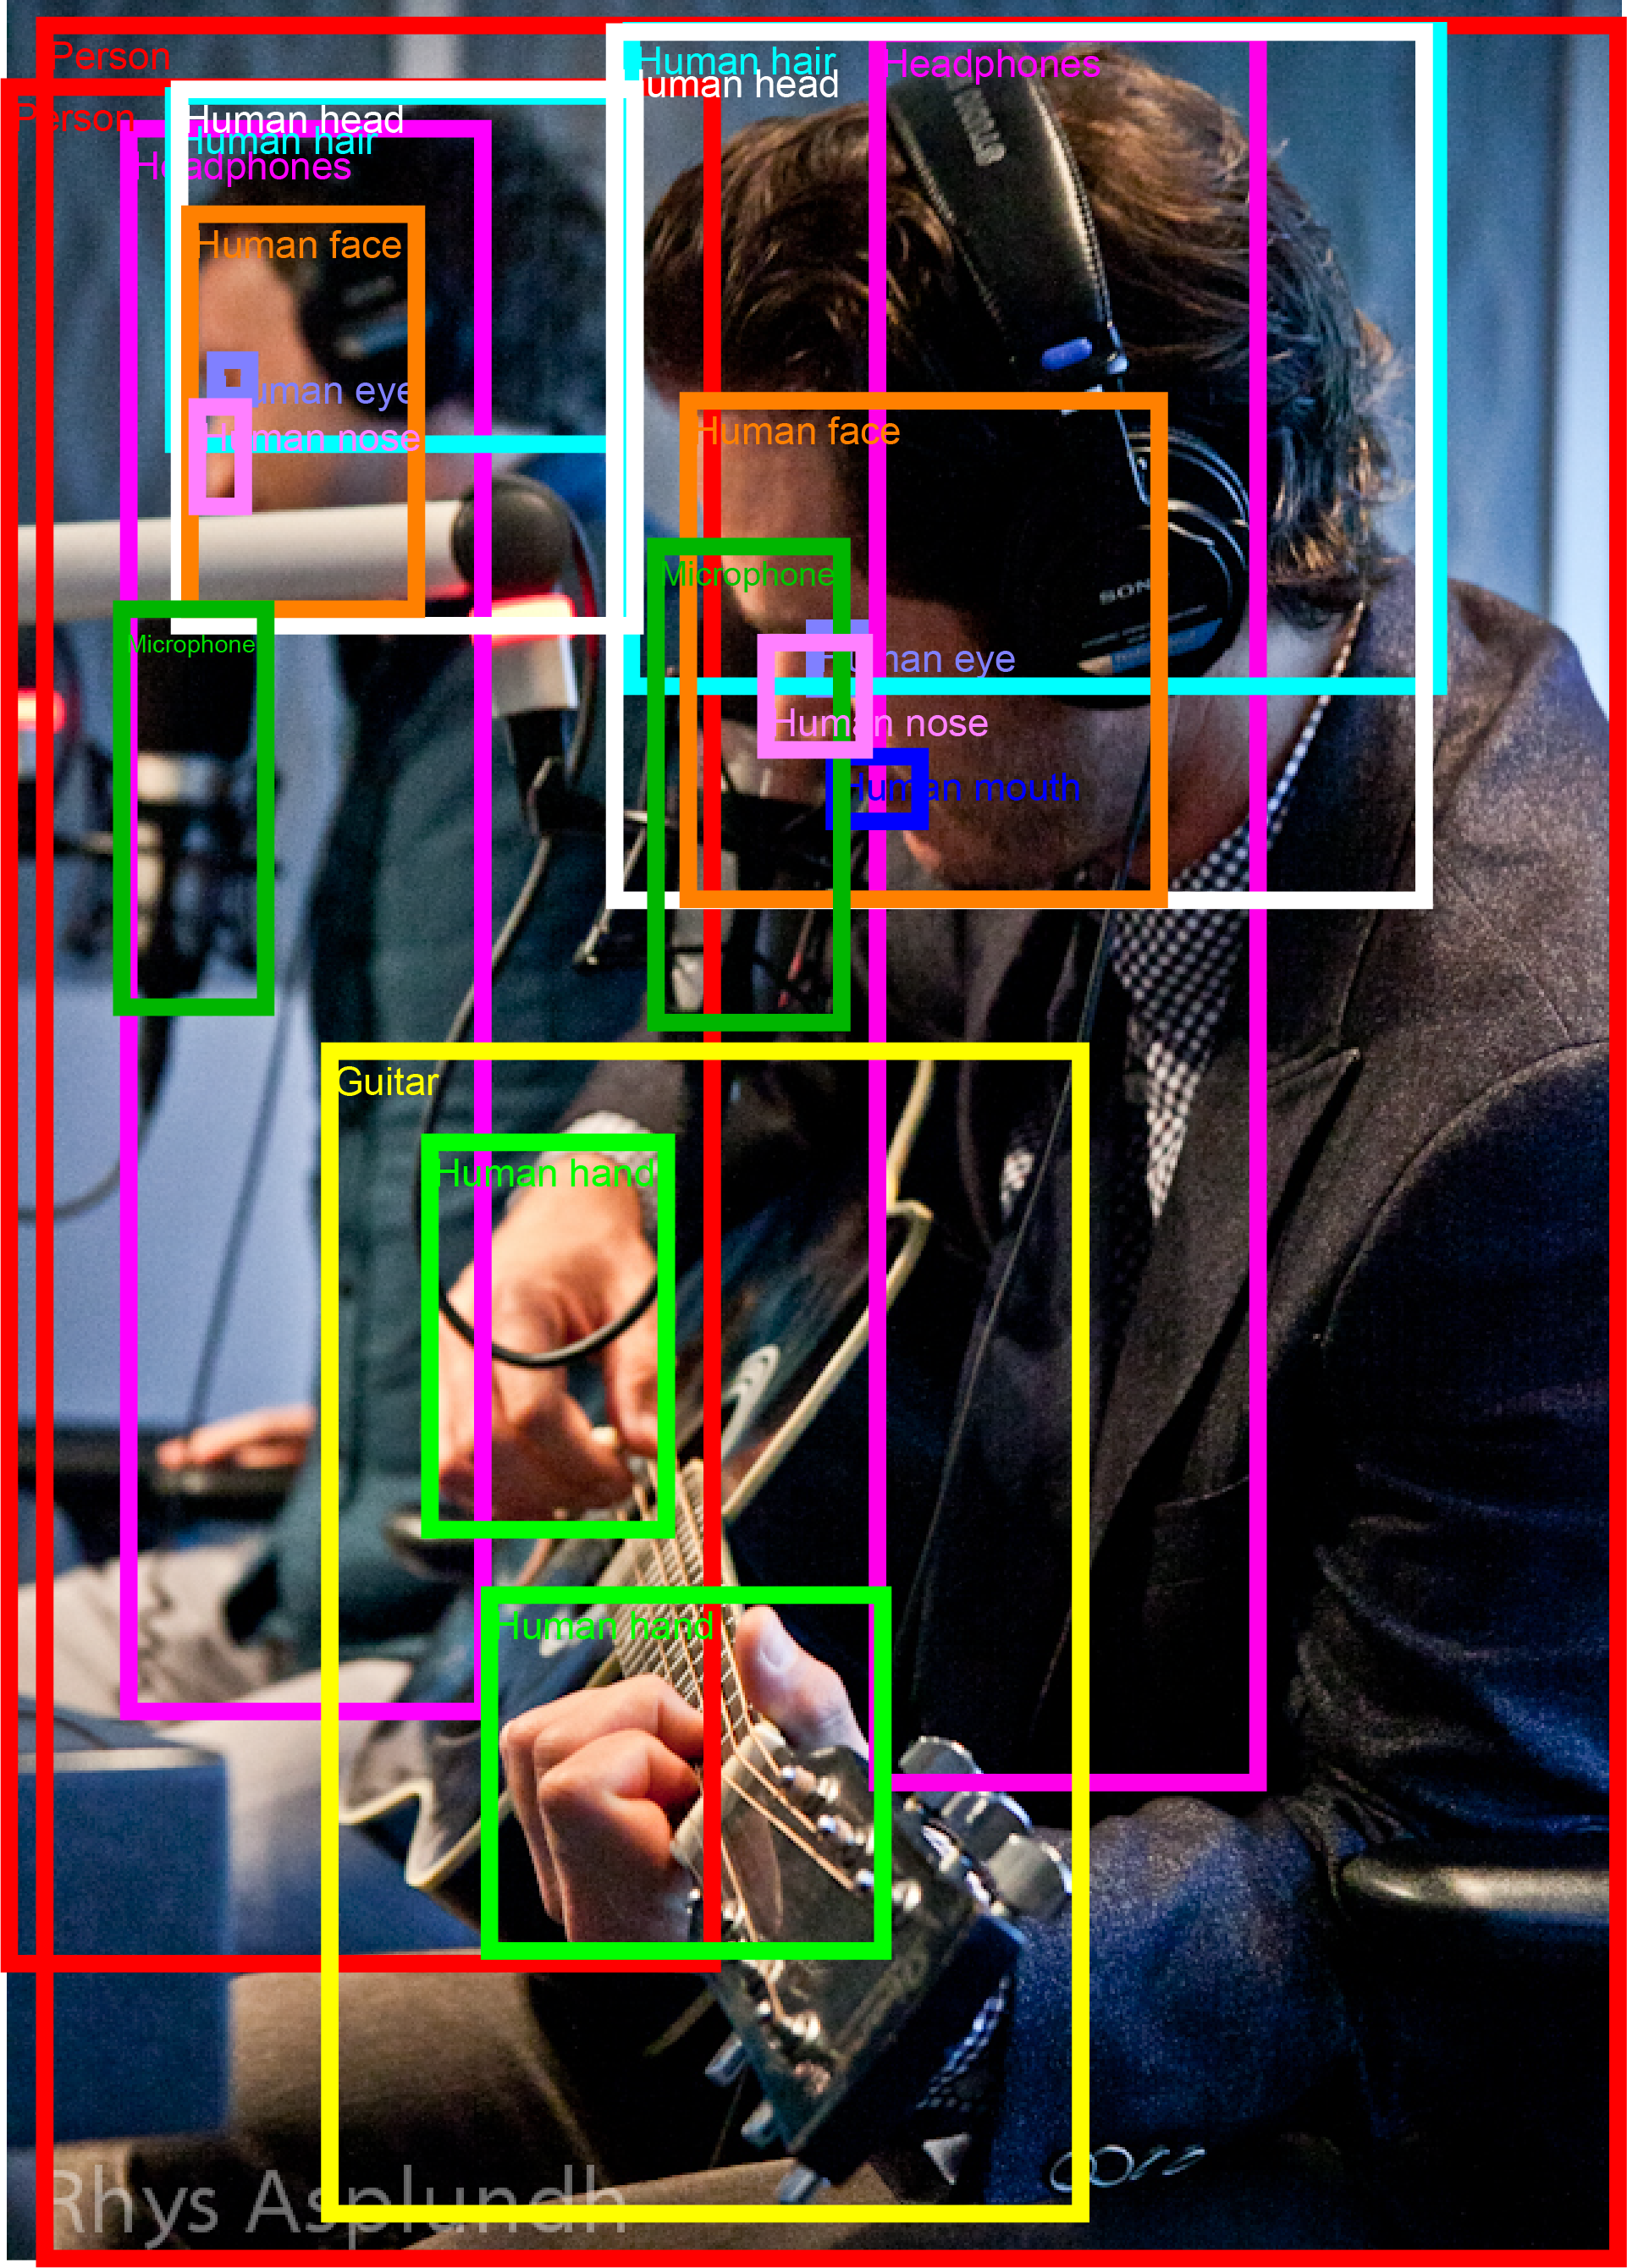
\includegraphics[width=.4\textwidth]{intro-1.png}
	\caption{\scriptsize Mark Paul Gosselaar plays the guitar by Rhys A. \cite{google:1}}
\end{figure}

The Kaggle competition created by Google \cite{kaggle} using a recently announced dataset is called Open Images 2019 - Object Detection\cite{google:1}, and it motivates this work. This project implements a strategy, using Deep Learning to solve the problem, which is grounded in some researches that this paper is going to present.

This project is a result of 3 months of research and hard work made in the area of computer vision and deep learning architecture. More than to solve the Kaggle problem, the main objective was learning about computer vision and more about Deep Learning.

\subsection{Problem Statement}

I want to start discussing the main difference between the proposal of the project and the final project delivered. When I wrote the proposal, I did not have the full context of the area, besides that, I proposed a possible and relevant architecture. The idea was to create a simple pipeline with two models concatenated, and each model would optimize one technique (classification and localization of bounding boxes). However, during more studying, it was clear that this architecture was burdensome and inefficient, which is not a problem for some circumstances, but this is not the case. Given that I have limited resources and time, and the dataset has around 1.7 million images, my proposal to use more than one models concatenated, knowing that I had to running the training process a few times, sounds very overwhelming, so I had to change my initial design.

We could define the object detection research area in two big sets about how to predict objects in an image. The first goes to path of pass the image for the model more than once to return one prediction. The computer vision area believed for much time that this was the only way. In the very beginning, there were very complex architectures using SVMs (Support Vector Machines) and regressors \cite{svm1}\cite{svm2} to draw bounding boxes. Nowadays, there are more robust architectures using deep learning like R-CNNs \cite{rcnn}, Fast R-CNNs \cite{fastrcnn} and Faster R-CNNs\cite{fasterrcnn}. The second one goes to a performance path and limits the model to pass the image just once to predict both, the bounding box localization and the classification, at the same time. Examples of this approach are YOLO (You Only Look Once)\cite{yolo} and SSD (Single Shot Detection) \cite{ssd}.

This project uses SSD structure, which will be detailed discussed in the next sections. At the very end, I am going to present the changes that were made in the architecture to use new networks (like Resnet and Xception) to extract more accurate data from the images.

\begin{figure}[!ht]
	\centering
	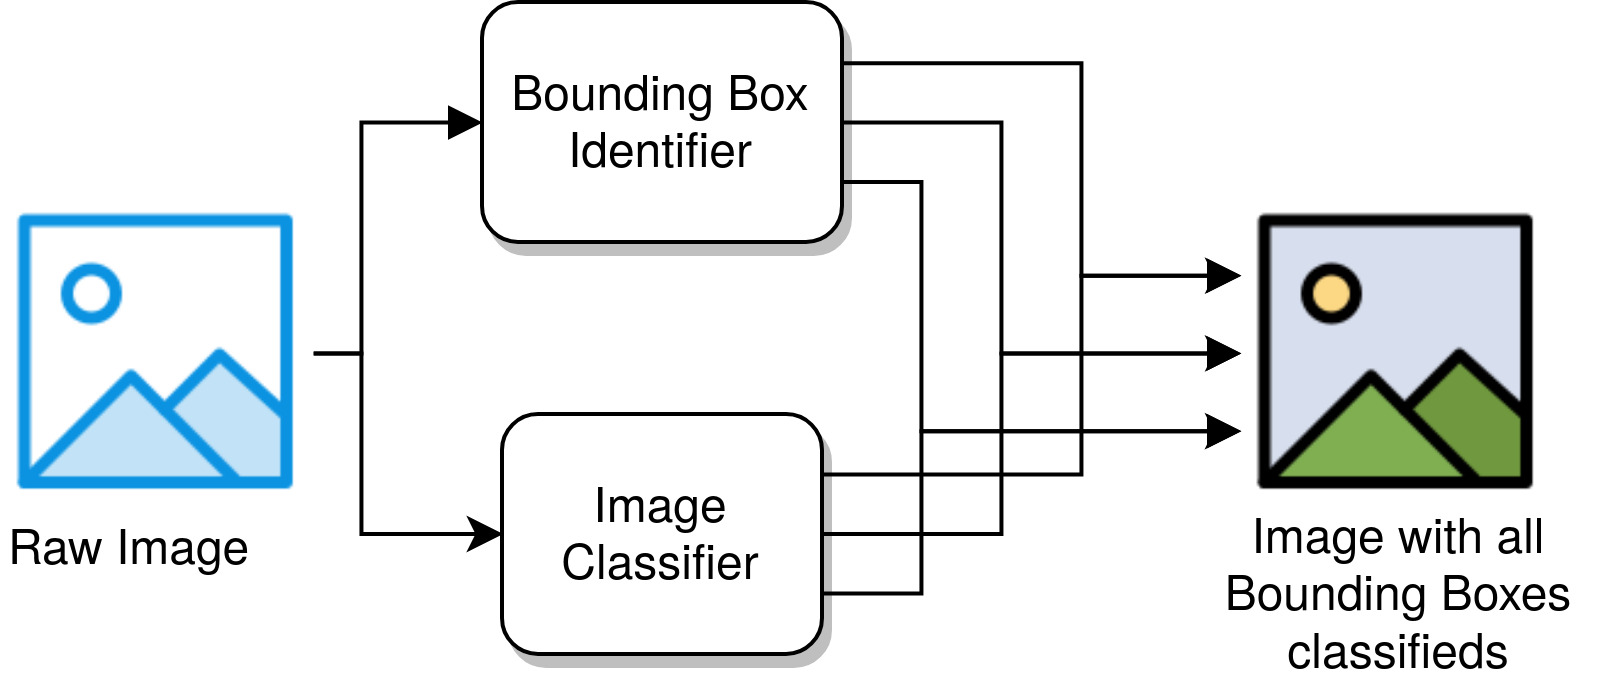
\includegraphics[width=.4\textwidth]{high-level-architecture.jpg}
	\caption{\scriptsize High level Model based on SSD idea}
\end{figure}

\subsection{Metrics}

The metric proposed by Google in the competition is the mean Average Precision (mAP) \cite{map}, a very didactic explanation about the metric could be found in here \cite{medium:1} and \cite{medium:2}.

The mAP metric could be defined as

{\centering
	\begin{equation*}
	mAP = \frac{\sum\limits_{c=1}^{C}AP_c} {C}
	\end{equation*}}

where $C$ value is the number of all categories (classes).

To understand $AP_c$, it must comprehend first what is $IoU$. $IoU$ is the Intersection over Union. It is equal to the ratio of the $Area\ of\ Overlap$ and the $Area\ of\ Union$, considering the Predict bounding box (created by the model) and the Ground-truth bounding box (previously annotated).


\begin{figure}[!ht]
	\centering
	\subfloat[\scriptsize  Difference between a Predict bounding box with a Ground-truth bouding box \cite{pyimage}]{{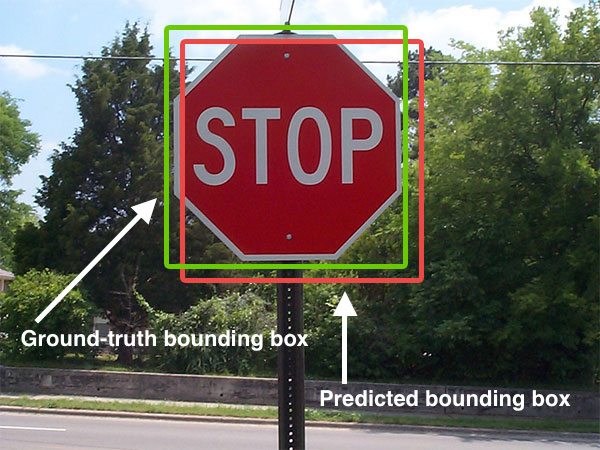
\includegraphics[width=5cm]{iou_stop_sign} }}%
	\qquad
	\subfloat[\scriptsize IoU visual represented \cite{pyimage}]{{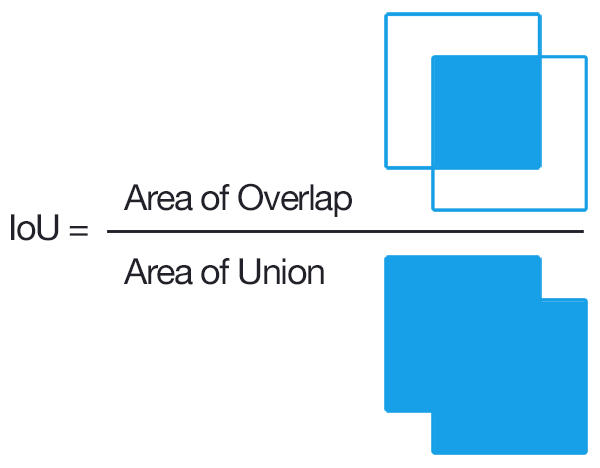
\includegraphics[width=5cm]{iou_equation} }}%
	%\caption{2 Figures side by side}%
	\label{fig:example}%
\end{figure}

Here, it is going to define:
\begin{align*}
True&Positive\ \dot=\ IoU > 0.5 \\
False&Positive\ \dot=\ IoU < 0.5 \\
&or\ DuplicatedPredictBoundingBox \\
False&Negative\ \dot=\ IoU > 0.5\ \\ 
&and \ WrongClassification
\end{align*}

With the concept of True Positive (TP), True Negatives (TN), and False Positives (FN) defined, it is possible to create a Precision-Recall Curve, which defines a function that gives a precision based on the recall.

\begin{figure}[!ht]
	
	\centering
	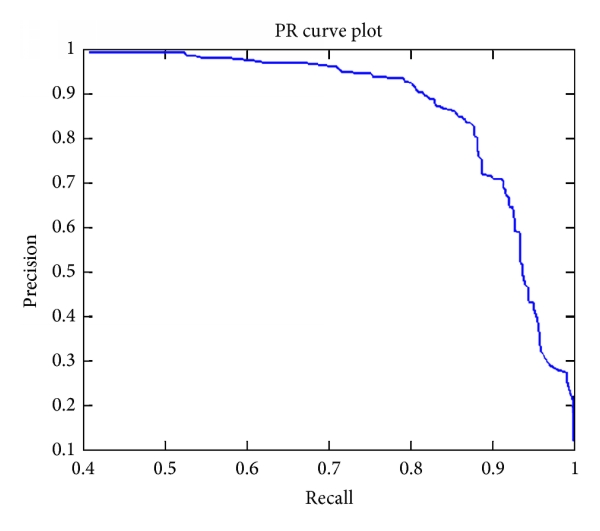
\includegraphics[width=.3\textwidth]{precision-recall.png}
	\caption{\scriptsize Precision-Recall curve \cite{medium:1}}
	
\end{figure}

So by definition, $AP_c$ (Average Precision of some category c), is defined as an Area Under the Curve ($AUC$) of the Precision-Recall curve.

{\centering
	\begin{equation*}
	AP_c = \int_{0}^{1} p(r) dr
	\end{equation*}
	where $p(r)$ is the precision defined in function of recall.}

It is essential to retain that in this project it is going to be used $AP_{50}$ (which uses a threshold of 0.5 in $IoU$ to define $TP$), but other average precision metrics could be used, like, $AP_{75}$ (with $IoU$ threshold of 0.75) or $AP_{90}$ (with $IoU$ threshold of 0.90).

\section{Analysis}

\subsection{Data Exploration}

For the problem itself, there are two datasets (Image-level and bounding boxes), plus two files that describe each class used in the labeling process, and the relation among them.

About the classes, there are 600 unique classes, and they are represented as a graph. So they have inheritances. All classes start from a class that I called "Entity" (it has no name, in fact), and all other classes derive from it or from the classes that derive from it on some level. \hyperref[sec:appendix-a]{In the appendix A}, I expose all connections at each level (the deepest level is five).

The Train, Cross-Validation and Test set are already given by Google. This project intends to use the same distribution given. However, during the analysis it was possible to notice that there are some classes presented in Train set that are not presented in Test and Cross-Validation sets. The following table shows how much unique classes are present in each data set.

\begin{table}[ht]
	\footnotesize
	\centering
	\caption{ \footnotesize Unique classes in each Dataset and amount of Bounding Boxes }
	\label{table1}
	\begin{tabular}{lll}
		& Unique Classes & Count of Boubing Boxes \\
		\rowcolor[HTML]{EFEFEF} 
		Train            & 599            & 14,609,671             \\
		Cross-Validation & 570            & 303,980                \\
		\rowcolor[HTML]{EFEFEF} 
		Test             & 583            & 937,327               
	\end{tabular}
\end{table}

Besides that, the distribution of each class is not uniform. 30 classes are responsible for 80\% of bounding boxes labels, and 300 classes are responsible for less than 1\% of bounding boxes. Of course, this affects how the final model performs in a random image.

\begin{figure}[!ht]
	\centering
	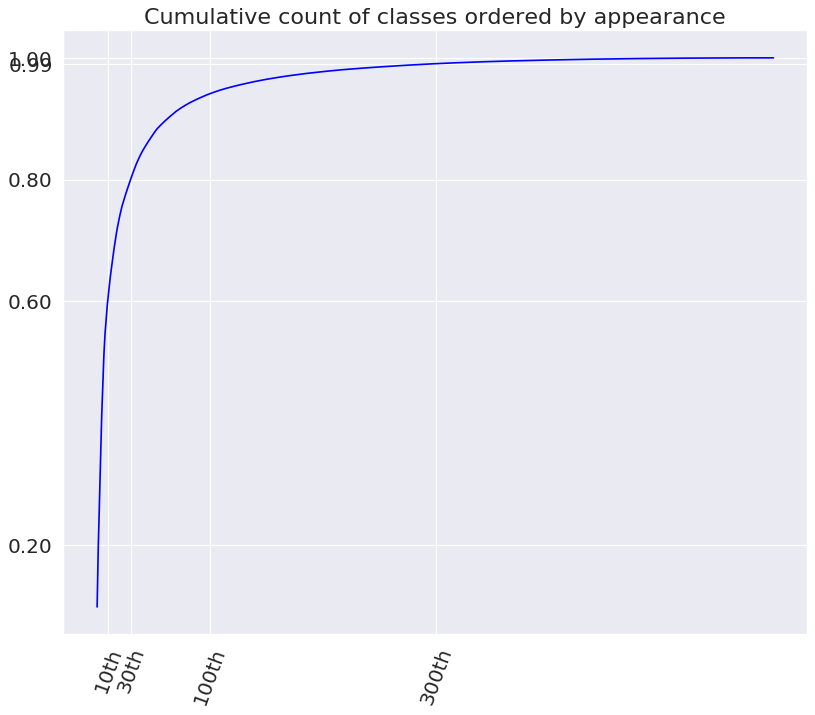
\includegraphics[width=0.5\textwidth]{cumulative-classes.png}
	\caption{\scriptsize Cumulative count of classes order by appearance}
\end{figure}

\begin{figure}[!ht]
	\centering
	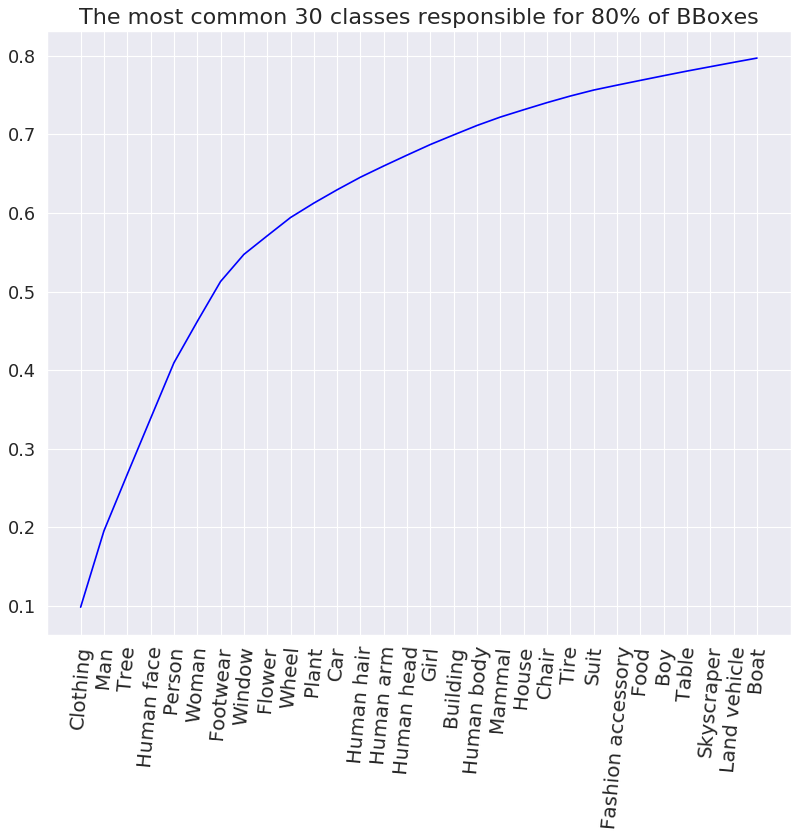
\includegraphics[width=0.5\textwidth]{30-most-frequently.png}
	\caption{\scriptsize The thirty classes with most appearance}
\end{figure}

The two datasets, image-level label and bounding boxes, both are divided in three (train, test, cross-validation). Google explains in the blog \cite{imgdataset} how they create the Image-level dataset and how, with it, they create the bounding boxes dataset. The label-image set was created, and a little part of it (around 1.7 million images) were chosen to have more granular work. The labels previously created were relabeled and transformed in bounding boxes that identify, not only what is the object, but the position of those objects. This work uses only the bounding boxes dataset.

About Bounding Box Dataset, some points must be concerned.
The labels in the original data set are encoded (probably to avoid mismatch and homonyms). In the analysis process they were converted to semantic labels (using a support dataset provided by Google). However, in modeling, it is going to use the encoded version. 

\begin{table*}[!ht]
	\footnotesize
	\centering
	\caption{ \footnotesize Amount of each flag in Bounding Box dataset }
	\label{table2}
	\begin{tabular}{llllll}
		& IsOccluded & IsTruncated & IsGroupOf & IsDepiction & IsInside \\
		\rowcolor[HTML]{EFEFEF} 
		Train            & 9,629,150  & 3,643,883   & 852,641   & 774,485     & 13,718   \\
		Cross-Validation & 134,497    & 69,698      & 26,360    & 14,181      & 2,200    \\
		\rowcolor[HTML]{EFEFEF} 
		Test             & 417,398    & 211,732     & 81,037    & 44,038      & 6,964   
	\end{tabular}
\end{table*}

Beyond the label and the bounding boxes position, the dataset also has some flags (IsOccluded, IsTruncated, IsGroupOf, IsDepiction, IsInside). These flags are very helpful to debug the decisions that a model does.

"IsOccluded" points a Bounding Box that has a type of obstruction in it, making it more difficult to be understandable.

"IsTruncated" points a Bounding Box that ends or starts in some edges of the image.

"IsGroupOf" means that the label given is about a group of things, and the bounding box is around all of those things.

\begin{figure}[!ht]
	\centering
	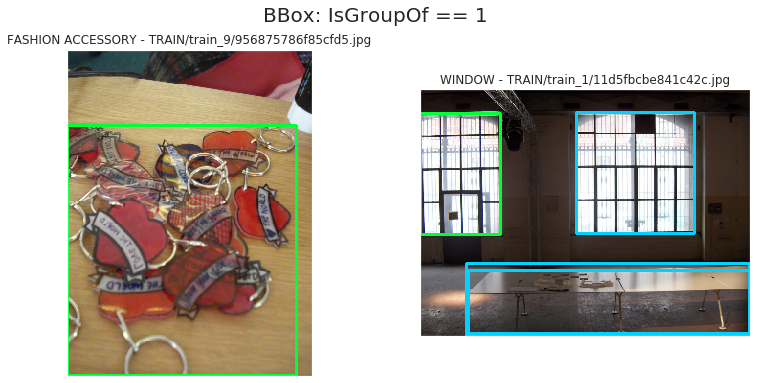
\includegraphics[width=.5\textwidth]{isgroupof-true.png}
	\caption{\scriptsize Bounding Box Green represents IsGroupOf True }
\end{figure}

"IsDepiction" represents bounding boxes that do not label the object itself, but a representation of the object. Draws, representation, costumes, are some examples.

"IsInside" is about the Bounding Boxes labeled inside rooms or buildings, with artificial light.

As stated, the distributions of classes are not uniform, and this is a big concern about how good the model will be. There is a more accurate and complete analysis made by me, with a study of the correlations between flags and many other topics in all datasets. It can be checked in here \cite{eda} on my github.

\subsection{Techniques}

This project is about how to design and to create deep neural networks. More than that, it is going to deep dive into how Convolutional Neural Networks (CNNs) work and how to extract more value of them.

Neural networks could have complex architectures made over some of straightforward ideas. First of all, there is the  function; the loss function is the measure of the error of some neural network, in this project it designs a tailor-made loss function (proposed by SSD paper), which I am going to discuss more further.

In the training process, we have to define a batch size. Batch size is a number which specifies how many examples we are going to use in the feed-forward process (the predict itself), and how many targets we are going to compare with the results. With the predictions in hand, we compare with targets previously labelled using the loss function. Then, in the process called backpropagation, it is used an optimizer to update the weights of the neural network.

To converge neural networks, for most of the times, we have to pass the same train set in the model, doing the feed-forward and backpropagation. The Epoch number defines how many times we are doing this. Besides running many epochs, sometimes, there is not enough data or data with quality to train a Neural Network. For that reason, we also have to do a process called data augmentation, which consists of augmenting the dataset with more useful examples created with the original ones.

Convolutional Neural Networks (CNNs)\cite{cnns} are neural networks with convolutional layers. These are layers that identify patterns in the images. In the first levels, they find the most common patterns, as edges, and in the deep levels, they identify the most specific patterns, as the form of a cat. These patterns are identified creating many filters and applying filters over filters to classify more complex patterns, we call this filters, kernels. Besides that, we condense the filters information applied in convolutional layers with pooling layers, which have the purpose of considering only the core information for the deeper layers. \cite{cnn:1} AlexNet \cite{AlexNet} was the first famous CNN architecture to classify images. Many others come later derived from it and newer ones, like VGG \cite{vgg}, ResNET \cite{resnet}, Inception \cite{inception} or Xception \cite{xception}.

\subsection{Benchmark}

This project was inspired by the Kaggle competition launched by Google, given that, It is going to use as a benchmark the leaderboard itself, \cite{leaderboard} and the goal is to achieve the best score that I can do, with the resources and the time that I have available.

The Score evaluated is the same discussed in the metric topic of the first part of this project. 

\begin{figure}[!ht]
	\centering
	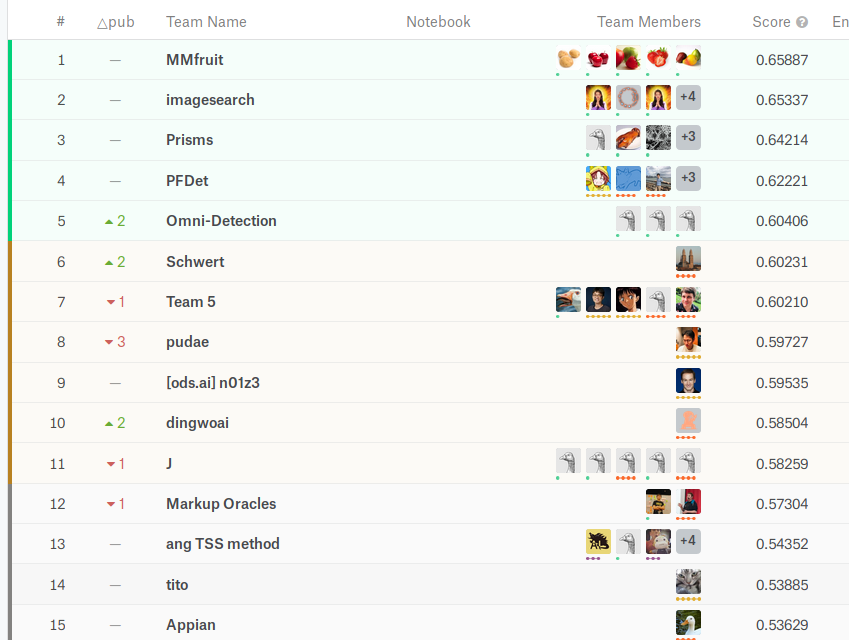
\includegraphics[width=0.5\textwidth]{leaderboard.png}
	\caption{\scriptsize Leaderboard Image Dection Kaggle Competition - 2019}
\end{figure}

\section{Methodology}

\subsection{Data Preprocessing}

There are three processes made in the data of this project. The first one is a simple One Hot Encode in the categorical feature that defines the class of the bounding box. One Hot Encode is a technique that maps a categorical variable to many boolean features, as many of the numbers of the categories. Each class is recorded as True in the category column created.

The second one is data augmentation. Because this dataset is hugely unbalanced, this project uses this approach to reduce the problem. It is defined five levels of data augmentations, as described below, and it is applied only one of that in each image of the dataset, based on how frequent is a class - more frequent is the class, lesser is the level. Each level creates newly enhanced images.

1st level - Image flip horizontally
2nd level - 1st level + randomly change the saturation 
3rd level - 2nd level + randomly change the contrast + flip horizontally with randomly change of saturation 
4th level - 3rd level + nine slight zooms in the image
5th level - 4th level + nine large zooms in the image

\begin{figure}[!ht]
	\centering
	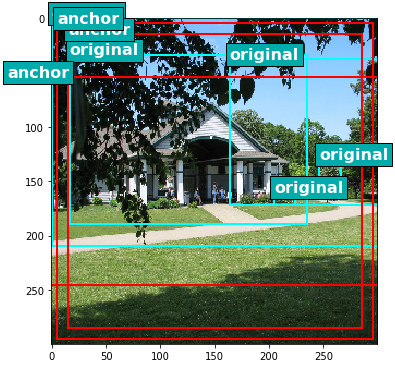
\includegraphics[width=0.5\textwidth]{original-img.png}
	\caption{\scriptsize Original Image with anchors (red) and original bboxes (blue)}
	\label{original}
\end{figure}

The SSD paper proposes the image flips and the zooms to augment the data. However, the saturation and contrast changes was an approach inspired by much reading on data augmentation process. By transforming the image with the contrast and saturation, the hypothesis was that the neural network would have different conditions to identify the objects. 

\begin{figure}[!ht]
	\centering
	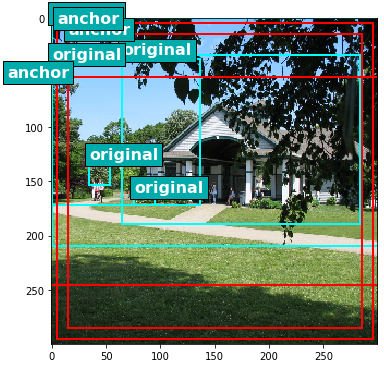
\includegraphics[width=0.5\textwidth]{flip-data-aug.png}
	\caption{\scriptsize Flip Image (data augmentation) with anchors (red) and original bboxes (blue)}
\end{figure}

The third and last process is data selection to train. The initial train dataset contains more than 1.7 million images, with more than 14 million bounding boxes. After data augmentation, this training dataset reaches 2.7 million images with more than 23 millions bounding boxes, which is more balanced, but it is enormous. This project created a subset of train dataset trying to preserve the proportions of the more balanced data, but making it possible to train each epoch in the available time. The data selection is described next. The train augmented dataset was divided into batches (around 50 images each), and by analysing them, the top 650 ones that contained the most balanced dataset were chosen.

All these processes comprehend many steps, and they are available in the GitHub \cite{balmeidas}.
\subsection{Implementation}

SSD is a technique which incorporates in the VGG16 a capability to find bounding boxes. To do so, it uses the concept of the convolutional layers. In the paper, they propose to remove the fully connected and final layers (which classifies the image overall) and to plug a new architecture. This architecture takes the last feature maps and applies into them a sequence of convolutions (actually, a set of two convolutions, which I am going to describe as a convolutional set). Each convolutional set reduces the features map and passes it to the next level. Also, it is used to predict an object in each kernel application of the present convolutional layer. Given that each set reduces the feature map, it increases for the next ones the length of the possible bounding box that could be predicted. So in the first levels of this architecture, the network predicts smaller bounding boxes, and in the final levels, the network predicts bigger bounding boxes.

For each kernel application, we also define some forms of bounding boxes, changing the proportion of the width and size based on the kernel. The paper defines these "default bounding boxes" as Anchors.

All kernels are squares, with 3x3 pixels of the feature map, and depending on the level there are 4 or 6 anchors inside this kernel. Two of them are squares with the proportion of height per width equals 1. The other two consider the proportion of height and width equals 2 and 1/2. And for the case of 6 anchors, another 2 proportions of height and width equals 3 and 1/3 are considered. With an input image with 300x300 pixels, the SSD predicts 8732 bounding boxes (one for each Anchor defined).

The shape of the predicted tensor for each of 8732 outputs is a tensor with n class + 4 position metrics of the bounding boxes (which SSD paper states to use the position x of the centre, the position y of the centre, width and height). In this project, the output tensor of this architecture have 3-rank, and its shape is (batch-size, 8732, (600+4)). 600 is the number of the classes in the Open Images dataset.

\begin{figure}[!ht]
	\centering
	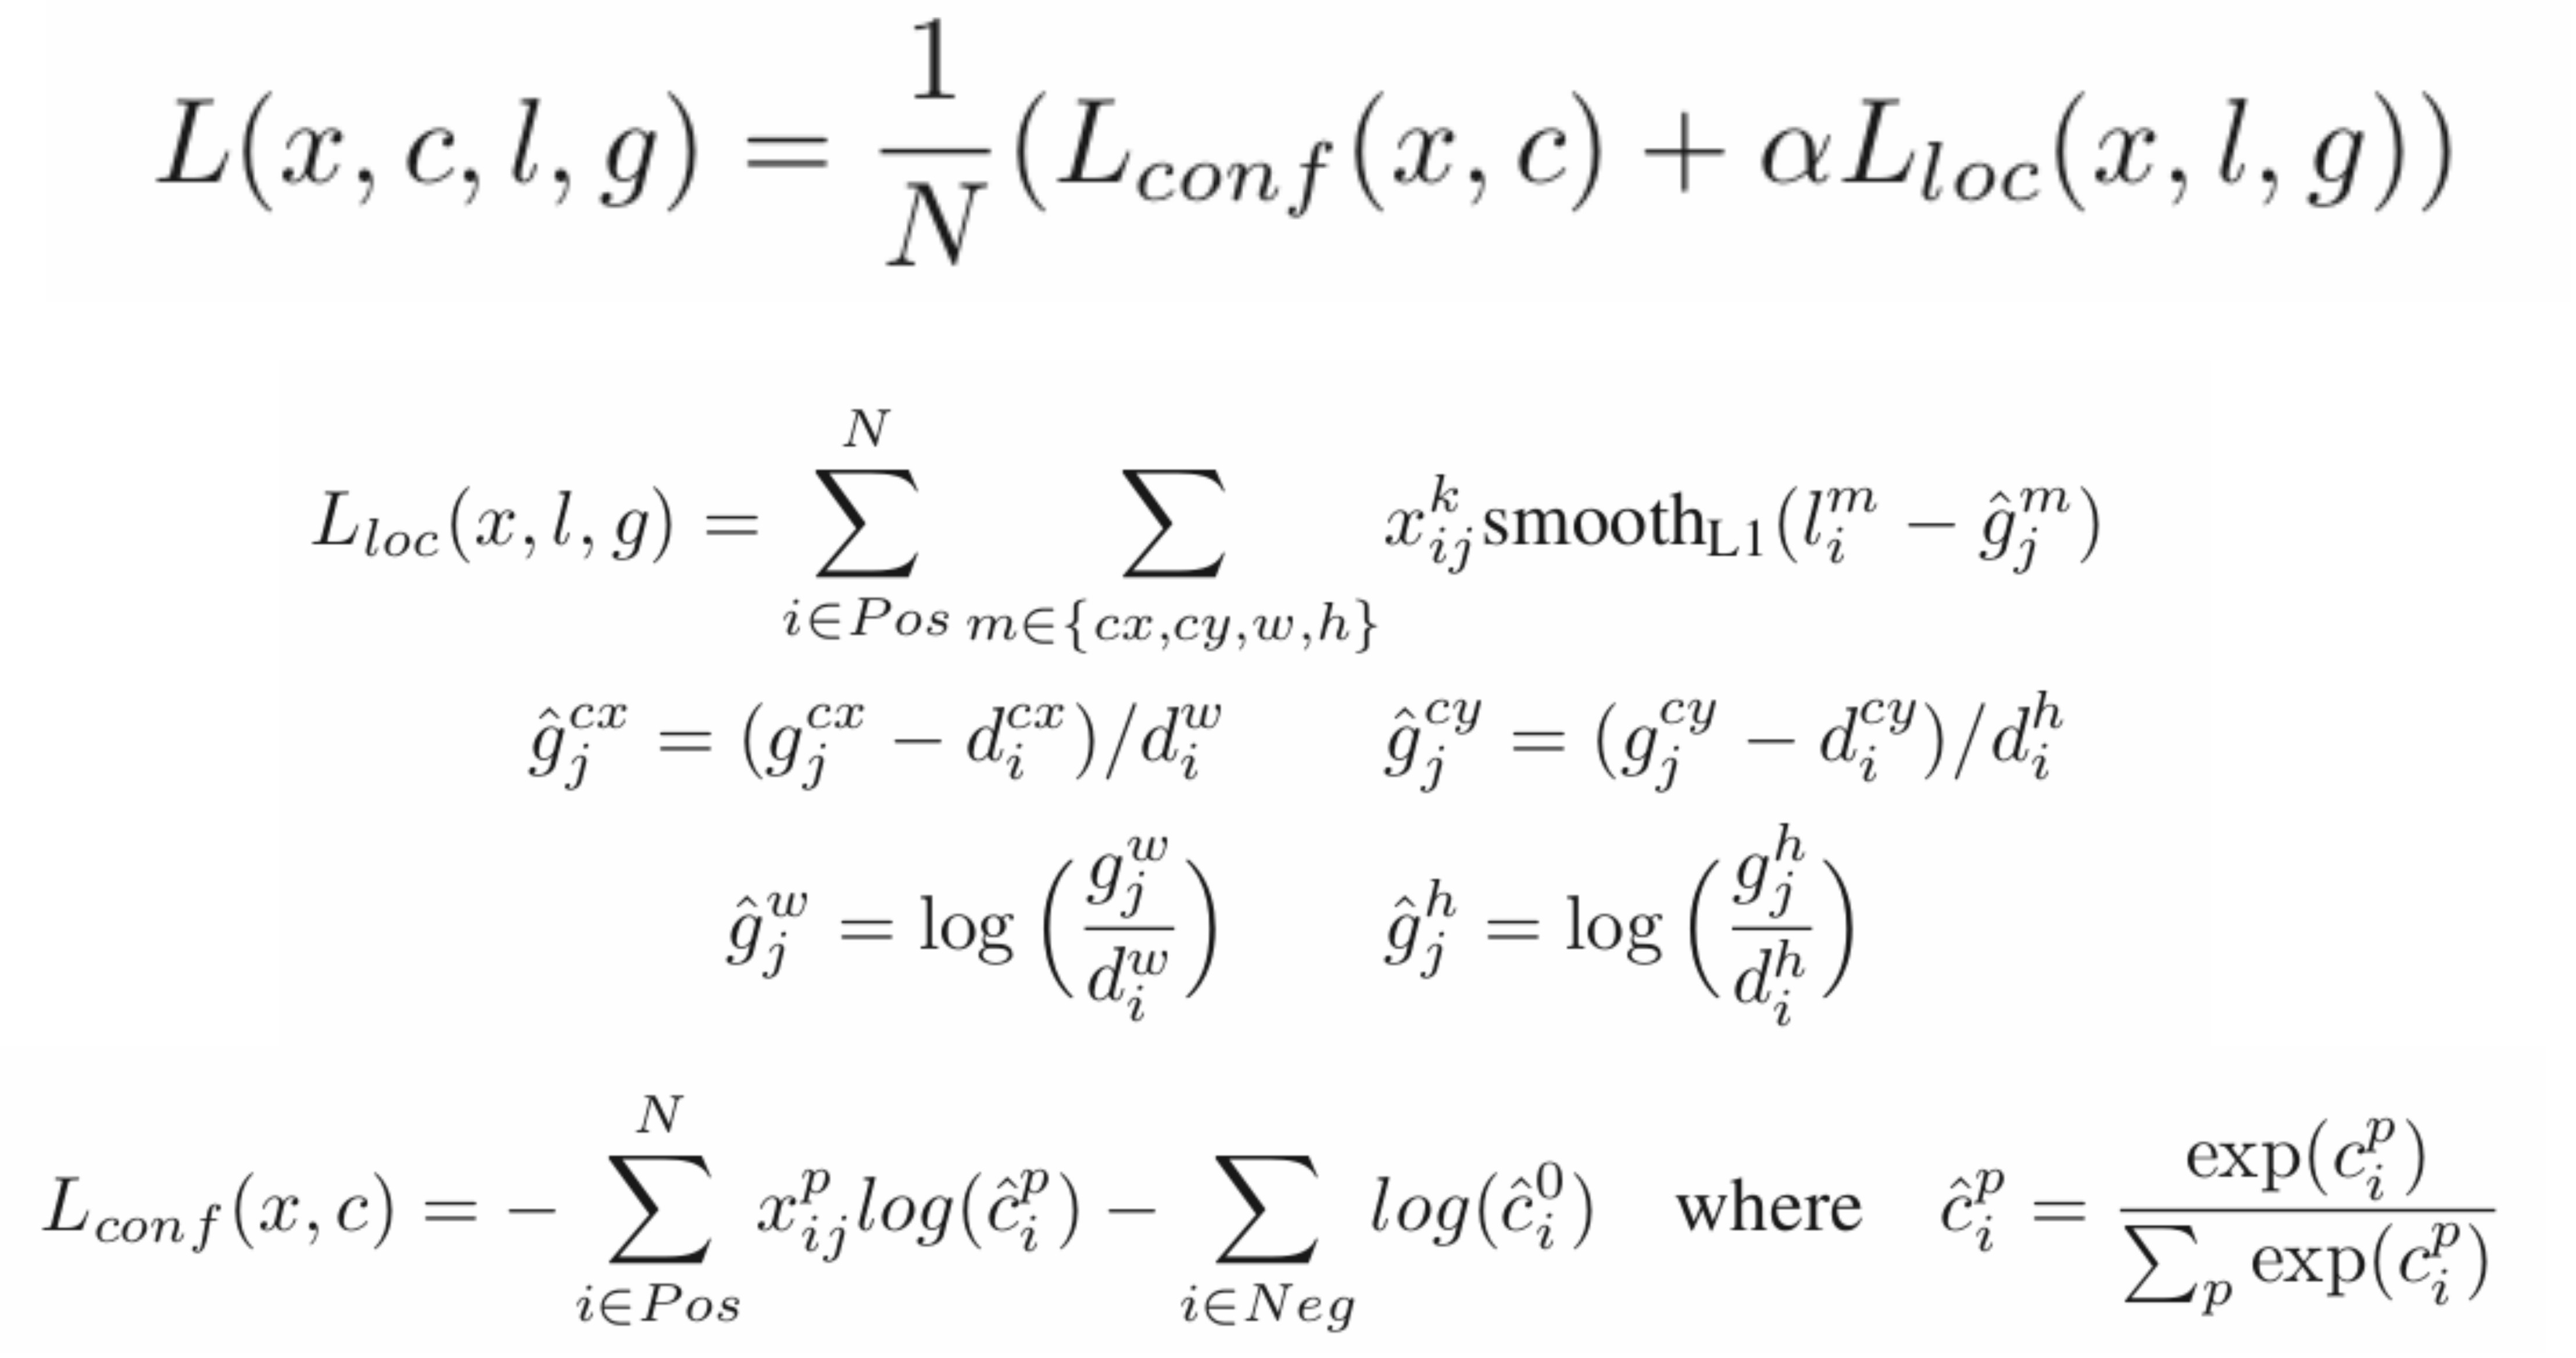
\includegraphics[width=0.5\textwidth]{loss.jpg}
	\caption{\scriptsize The tailor-made implementation \cite{losscode}}
	\label{losscode}
\end{figure}

To evaluate this, the SSD paper proposes a loss function which mixes the classification loss, using log loss function in softmax of each class and a regressor error metric, summing both.

After that, it was designed a custom Keras layer to the network for when it operates in the inference mode. This layer intends to suppress these 8732 bounding boxes using non-max-suppression with IOU threshold of 0.45, keeping the 200th most relevant bounding boxes with the higher evaluated metrics.

\begin{figure*}[!ht]
	\centering
	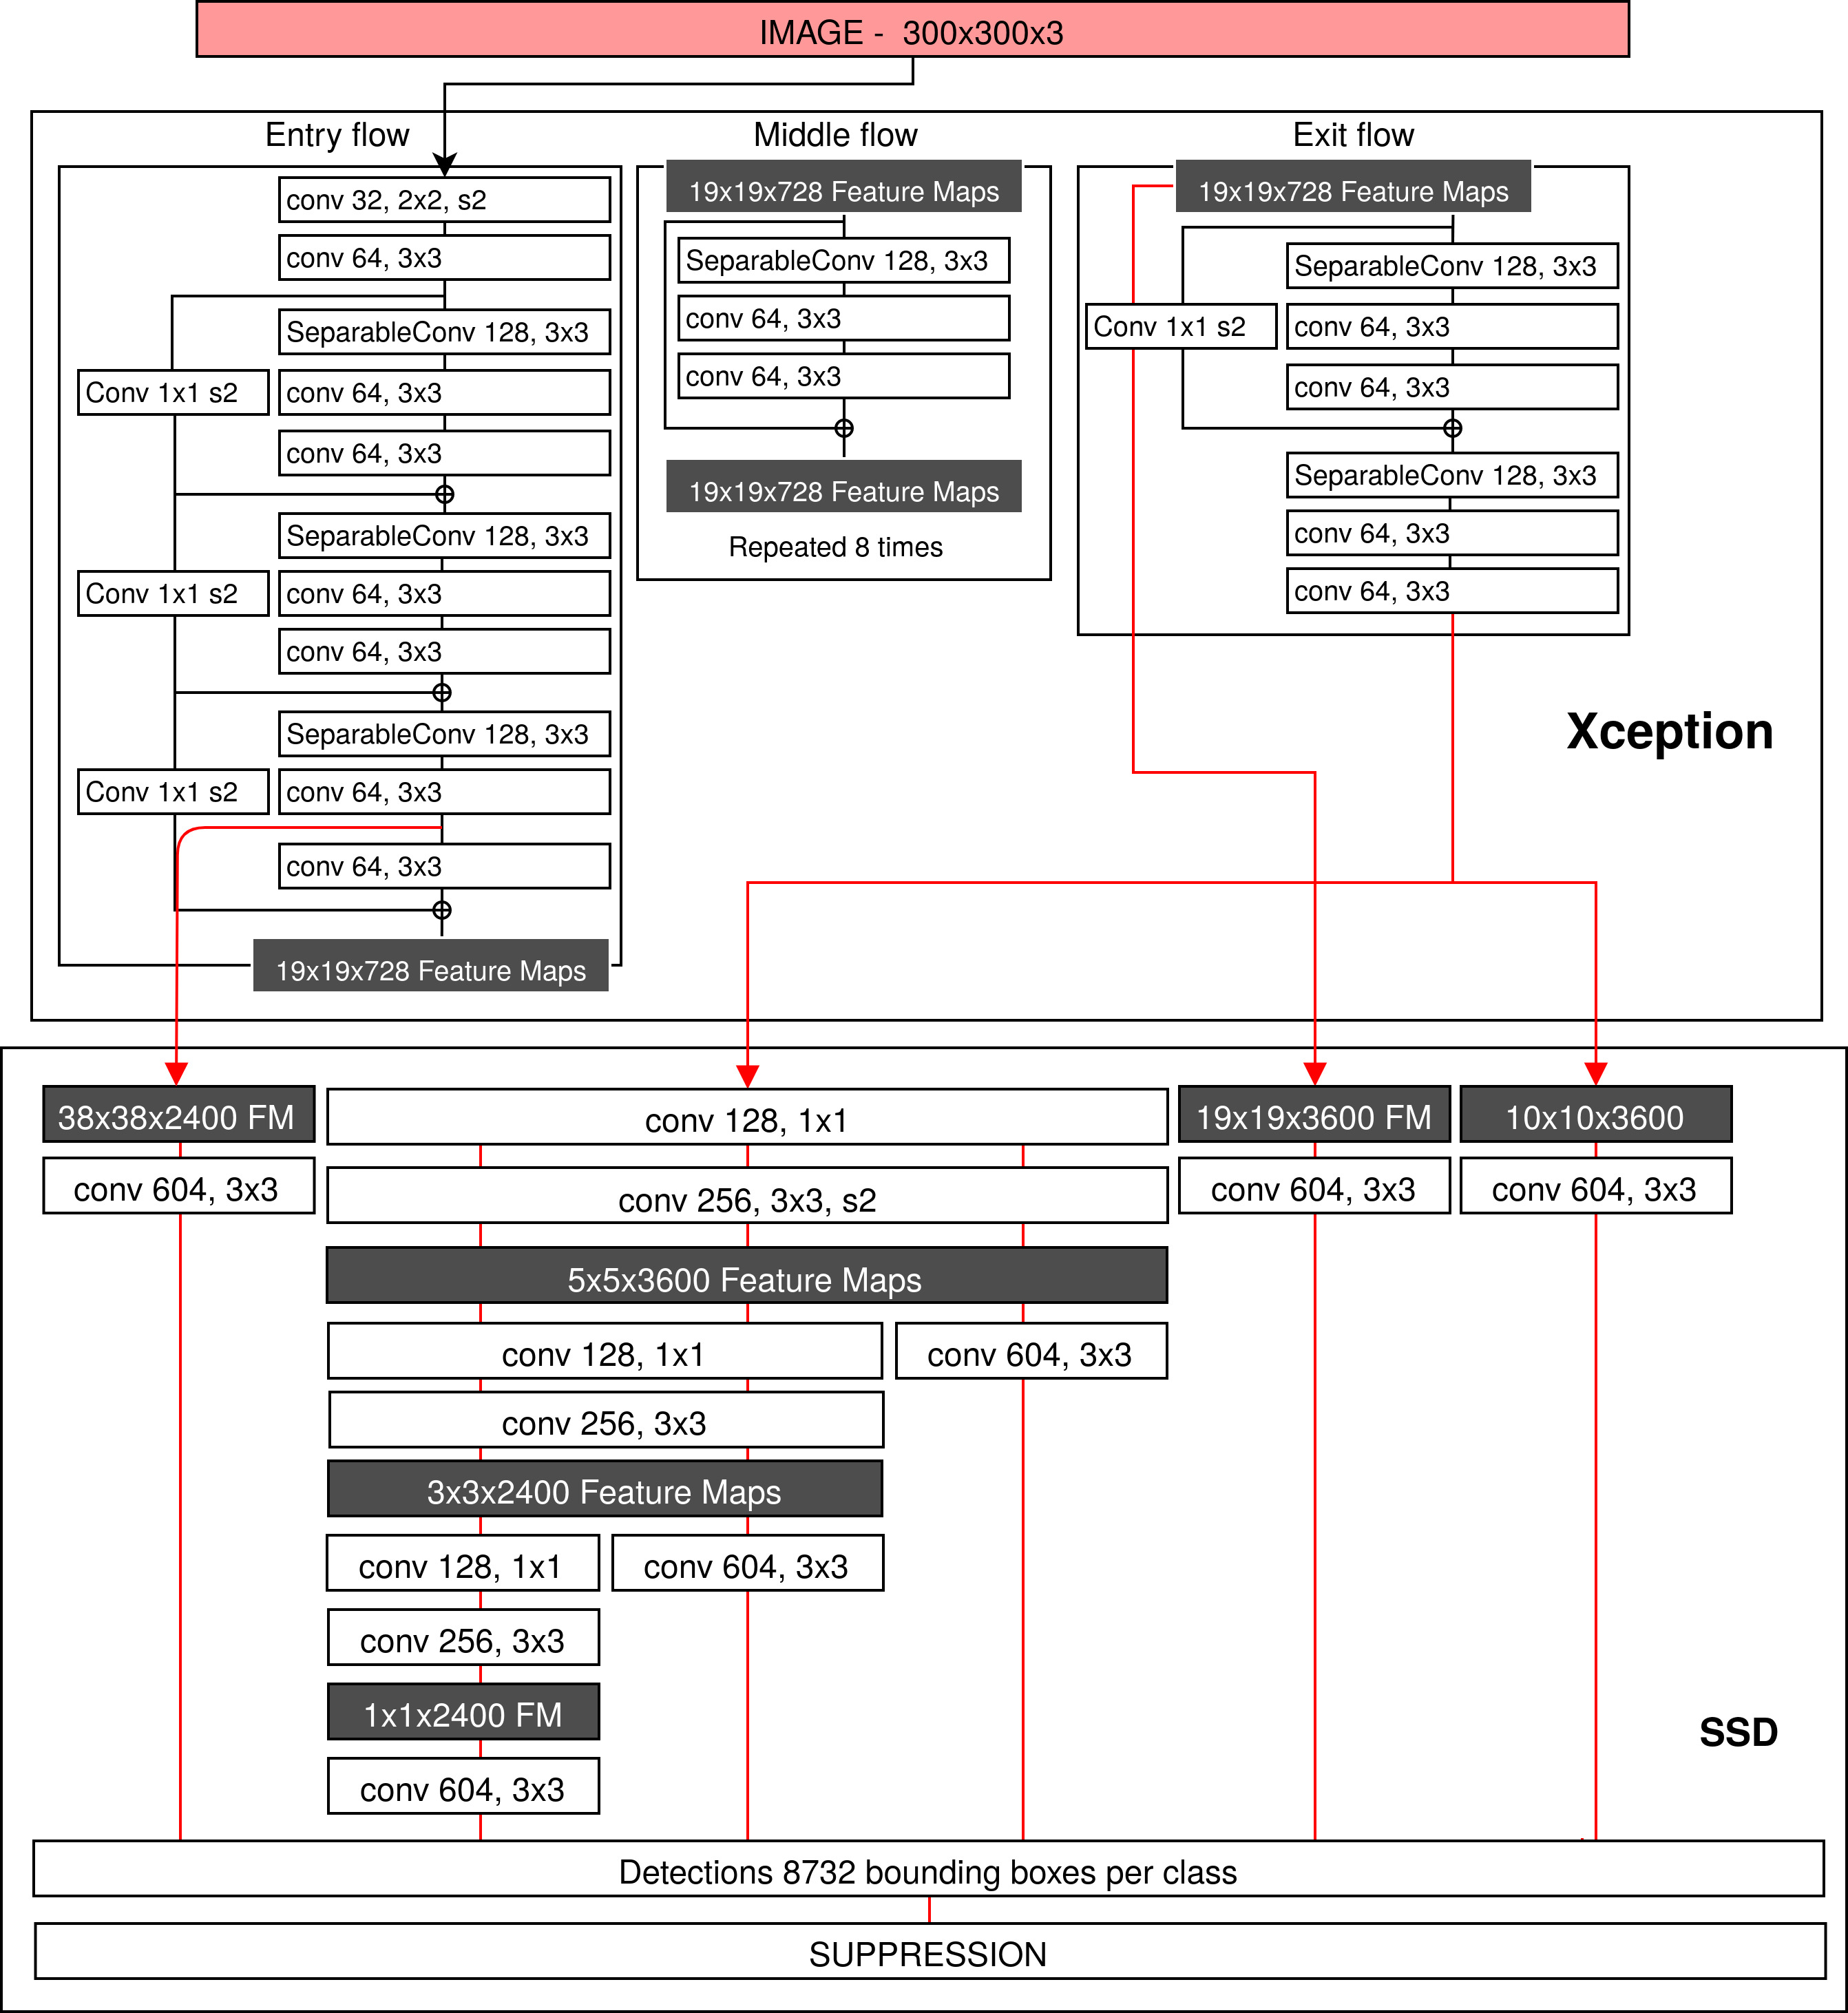
\includegraphics[width=0.9\textwidth]{xception+ssd.jpg}
	\caption{\scriptsize Final Model - SSD + Xception}
	\label{architecture}
\end{figure*}

The first part of the research I spent designing the SSD as is, using Keras and Tensorflow. The architecture developed is the same proposed in the paper. The full code is available on Github \cite{balmeidas}. 

\subsection{Refinement}

After implementing the SDD with VGG16 as the paper proposes, I decided to change it and plugged three other networks at the start of the SSD structure, substituting VGG. The other ones are Mobilenet-v2, Resnet50 and Xception.

Each network used weights optimized in the training of the Imagenet dataset as an initial state, and the training process iterated over them, instead of entirely initial randomly weights.

In the Evaluation Section are the metrics collected in the cross-validation dataset for each architecture. Still, I decided to show and explain more about the winner, that was the Xception with SSD model.

To understand Xception, we have to understand depthwise separable convolution, which is simply the concept of a channel-wise spatial convolution (which is a convolution not only in the feature map but among the channels) concatenated with a 1x1 convolution called pointwise convolution. These 1x1 convolutions could be understood as a type of pooling over the channels, and they intend to reduce the number of channels. The Xception proposes to revert the order of the depthwise convolution with the 1x1 convolution. The main argument is that this reduces the weights of the model considerably with the same accuracy.

\ref{architecture} illustrates what this project implements, plugging the first architecture proposed in Xception with its depthwise-pointwise.

\section{Results}

\subsection{Model Evaluation and Validation}


To the final results, many models were trained. All of them followed the same pattern, they used the partial train dataset created, the 35k images (650 batches of 50 images), and they were evaluated in the cross-validation dataset. The hyper-parameters used to train the models were: the amount of epoch was 30, with a batch size of 24, SGD (Stochastic Gradient Descent) as the optimizer, with momentum of 0.9, decay of 0.0005 and a learning rate scheduler that uses $10^-3$ in first 15 epochs, $10^-4$ in the epochs 16 to 25, and $10^-5$ in the last five epochs.

This work presents the best four models created with this evaluation model. The cross-validation dataset has 570 classes, table \ref{table:crossvaltable} are the mAP achieved for each model, I also considered the weighted mAP, which is the weighted mean AP, and the weights are the amount of the bounding boxes of each class. The weighted mAP is calculated because the dataset is very unbalanced \cite{modeleval}.

% Please add the following required packages to your document preamble:
% \usepackage[table,xcdraw]{xcolor}
% If you use beamer only pass "xcolor=table" option, i.e. \documentclass[xcolor=table]{beamer}
\begin{table}[!ht]
	\begin{tabular}{lll}
		\rowcolor[HTML]{EFEFEF} 
		Architectures & Standard & Weighted \\
		VGG16+SSD     & 0.0012 & 0.0002   \\
		\rowcolor[HTML]{EFEFEF} 
		Mobilenet+SSD & 0.0036 & 0.0020   \\
		\rowcolor[HTML]{FFFFFF} 
		Resnet+SSD    & 0.0091 & 0.0308   \\
		\rowcolor[HTML]{EFEFEF} 
		Xception+SSD  & 0.0174 & 0.1199  
	\end{tabular}
	\caption{mAP and weighted mAP for each final model}
	\label{table:crossvaltable}
\end{table}

The two best architectures, Resnet50 and Xception, were reloaded with the weights obtained and retrained for more 30 epochs. And the table \ref{table:finalchosenmodel} shows the final results in the cross-validation

\begin{table}[!ht]
	\begin{tabular}{lll}
		\rowcolor[HTML]{EFEFEF} 
		Architectures & Standard & Weighted \\
		Resnet+SSD v2 & 0.0067 & 0.0353   \\
		\rowcolor[HTML]{EFEFEF} 
		Xception+SSD v2 & 0.0229 & 0.1788
	\end{tabular}
	\caption{mAP and weighted mAP for the final two trained with more 30 epochs}
	\label{table:finalchosenmodel}
\end{table}

According to the evaluation made on cross-validation the Xception architecture with the SSD is the best model. A final evaluation in test set is made and REF show the final metric.

\begin{table}[!ht]
	\begin{tabular}{lll}
		\rowcolor[HTML]{EFEFEF} 
		Architectures & Standard & Weighted \\
		Xception+SSD v2 & 0.0256 & 0.0823
	\end{tabular}
	\caption{mAP and weighted mAP for the final model chosen with test dataset}
	\label{table:finalchosenmodel}
\end{table}

At the end model performs a 8.3\% for weighted mAP and 2.56\% for standard mAP. The weighted is about 12\% the first Kaggle submission and the Standard mAP is about 3.5\% of its achieved metric.

\subsection{Justification}

The final model, considering the weighted mAP tell us that it predicts correctly 8.3\% of the bounding boxes presented. The ultimate metric is a reasonable result, even predicting very poor for some classes, which is easy to conclude with the difference between weighted and standard mAP. The main reason for this is the unbalanced dataset.

After all, this reflects the types of pictures that this model is going to evaluate. How many are the images with crabs passing to the model in comparison with images of people?

I believe that filtering the dataset and working with fewer classes and balanced occurrences results in a much better model.

It is not recommended to use a model with this mAP on a critical system, like self-driving cars. But for a mobile application used to identify objects in user photos, it is an acceptable MVP (Minimum Viable Product), even more, if the project reduces the classes scope to recognize fewer categories.

\section{Conclusion}
\subsection{Free-Form Visualization}

\begin{figure}[!ht]
	\centering
	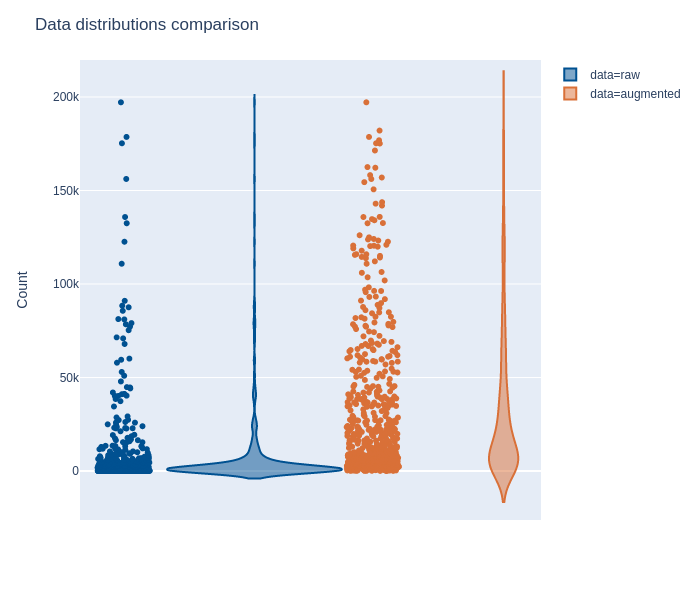
\includegraphics[width=0.5\textwidth]{data-aug2.png}
	\caption{Count amount of distribution for each class}
	\label{fig:aug2}
\end{figure}


As mentioned, the main challenge of the project is the unbalanced data. In this notebook, I demonstrated the criteria of the data augmentation. A good visualization that emphasis the distribution before and after data augmentation are \ref{augincreased} and \ref{fig:aug2}. The raw data has a more skewed distribution and clearly the data augmentation helped to fixed that as much as it could, the impact in the final model is expressive because of that.


The data augmentation itself is also a great part of the project. All the code to do the transformation are tailor-made and they could be found in github \cite{dataaugcode}. More examples of data augmentation made for \ref{original} are \ref{aug1plus} and \ref{aug2plus} applying zoom and control saturation.

\begin{figure}[!ht]
	\centering
	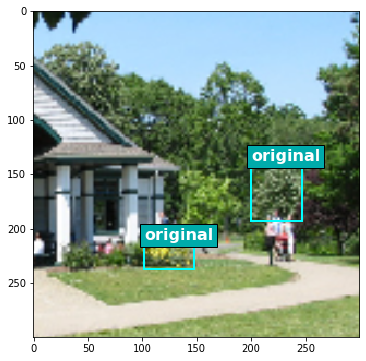
\includegraphics[width=0.4\textwidth]{aug-plus1.png}
	\caption{Zoom in data augmentation, transforming also the bounding boxes}
	\label{aug1plus}
\end{figure}

\begin{figure}[!ht]
	\centering
	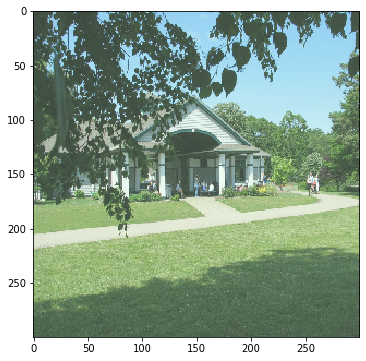
\includegraphics[width=0.4\textwidth]{aug-plus2.png}
	\caption{An example of saturation change}
	\label{aug2plus}
\end{figure}

\begin{figure*}[ht]
	\centering
	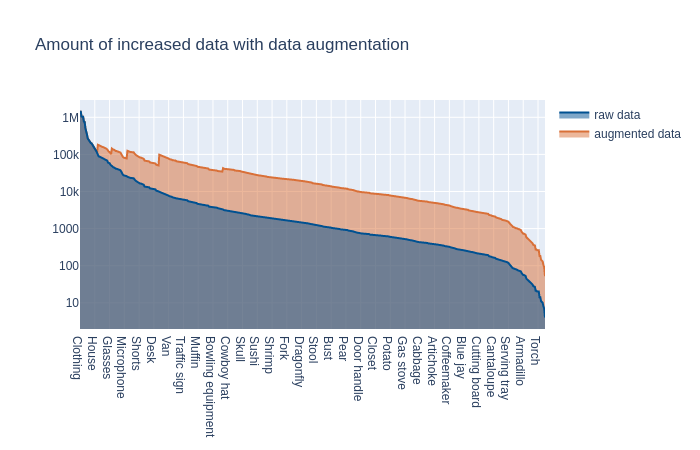
\includegraphics[width=1\textwidth]{data-aug1.png}
	\caption{Amount of data before/after data augmentation}
	\label{augincreased}
\end{figure*}

\subsection{Reflection}

In the very end, the final results are far from the top 50's Kaggle submissions, even the weighted mAP in the Xception with SSD.

The first reason is that the area of computer vision and object detection have a massive amount of knowledge and papers to read, and I am a rookie person is this area yet.

Another point that must be mentioned is the volume of data. The data is massive, and the impact of that is it needs many computer resources. To achieve these results, I created a lot of intermediates preprocess data, but also I filtered and removed a lot of data trying to evaluate and iterate faster. In the very end, I had 2.5 terabytes of hard drive used on my machine.

The final models were trained with a few parts of the dataset, around 35000 images (650 batches with approximately 50~55 images per batch). However, each one trained with 30 epochs spent more than 30 hours in Geforce 1080TI with 11Gb GDDR6. It is possible to estimate that this same train in the CPU would spend more than 120 hours.

More than one model was created. And each model created, each design proposed, each concept tested to fully understand the Networks consumed resources and time. It was three months on this project, and if I could, I would spend three more months improving it (and I probably will). To deliver a result in the due date, I decided on a strategy and followed it until the end.

Even the low score, I am very proud of this work. All code was designed by me and can be found in my Github, and a lot of knowledge from object detection to TensorFlow 2.0 and Keras was learnt.

\subsection{Improvement}

As previously stated, the dataset provided in the Kaggle competition is very unbalanced. This project used data augmentation technique to reduce this problem. However, there is plenty of room for more improvements in this aspect. The dataset has some flags, discussed in the data exploration section. These flags describe images that have objects with obstruction, images that are related to groups of objects and even images that are depictions, for example, a statue as a depiction of a human body. During the selection of the data to compose the subset for training the networks, these flags can be used to guarantee a more balanced data. The impact of this in the model would be better predictions since the network is trained with more data for the classes that have fewer bounding boxes.

Another improvement would be running the training process for more epochs. In this project, the models trained with a maximum of 60 epochs, because the time is limited. Though, the SSD paper proposes around 200 epochs. This improvement would impact directly on the mAP metric, increasing how much the model learned to predict.

Last, but not least, as discussed before, there are other types of Convolutional Neural Networks. YOLO can be used to attempt to solve the problem. It uses an entirely different architecture but could be a compelling approach to compare YOLO and SSD using this dataset since the papers related to this project compare them using much smaller datasets. The idea behind this change in the architecture would be increasing the object detections in the images as well.

\clearpage
\bibliographystyle{unsrt}
\bibliography{references.bib}{}

\begin{appendices}
	\label{sec:appendix-a}
	\section {Class hierarchy}
	
	\begin{figure*}[!ht]
		\centering
		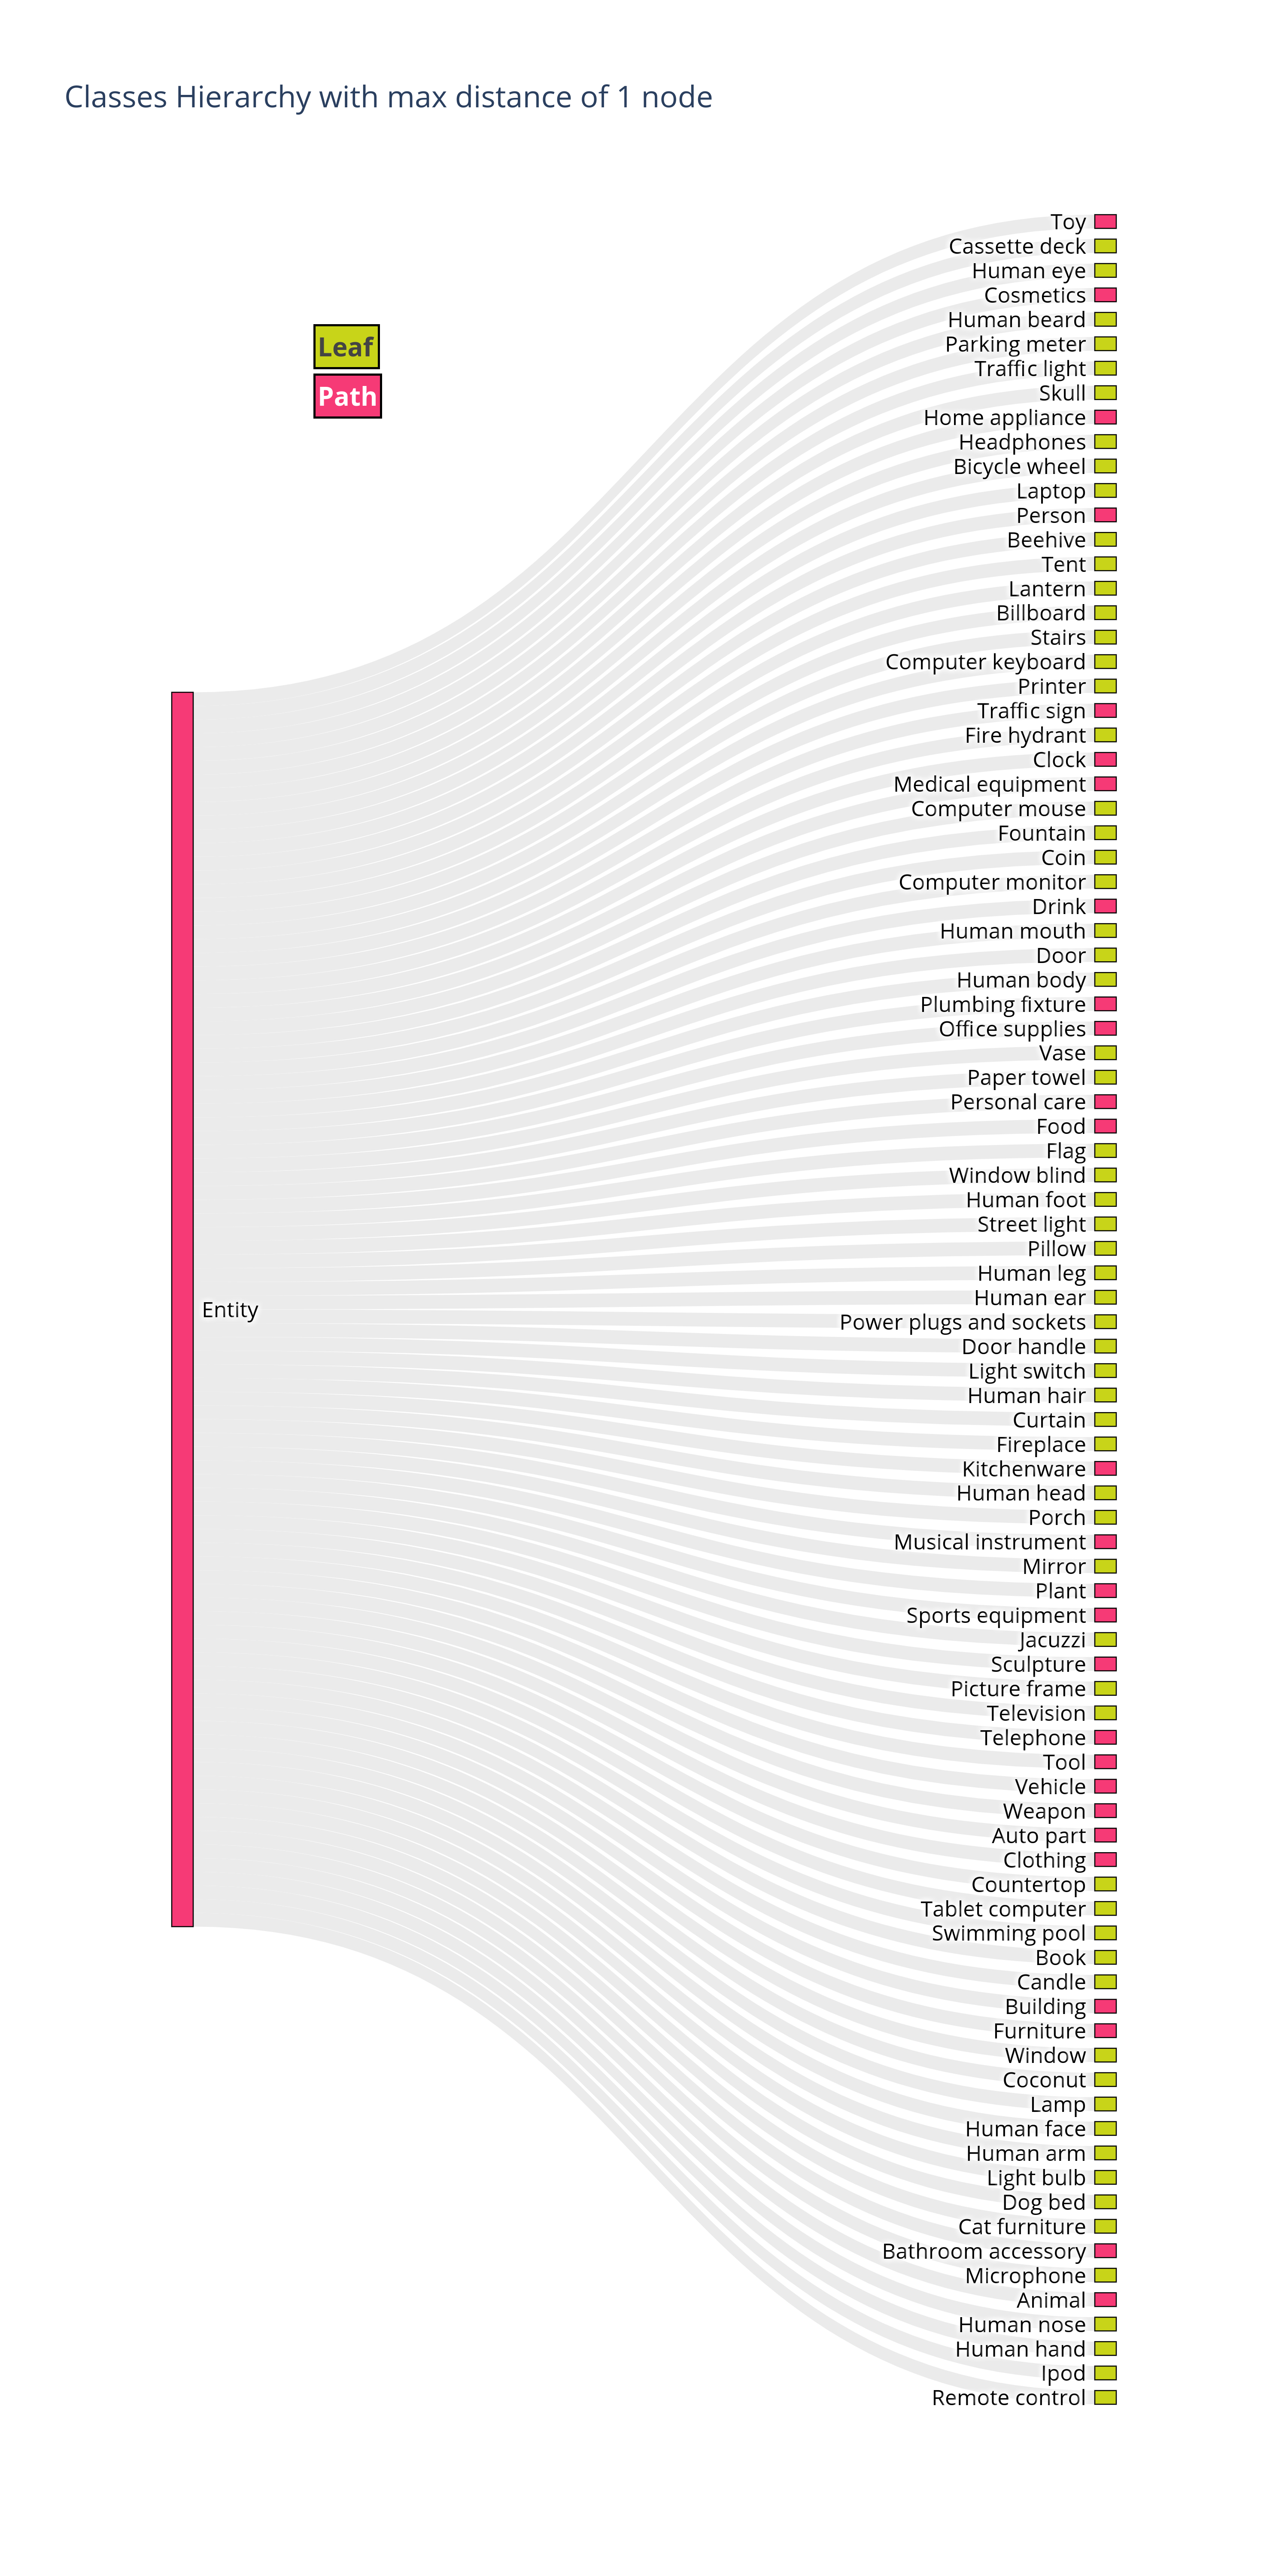
\includegraphics[width=0.7\textwidth]{lvl1_classes.png}
		\caption{\scriptsize Class Hierarchy - First Level}
	\end{figure*}
	
	\begin{figure}[!ht]
		\centering
		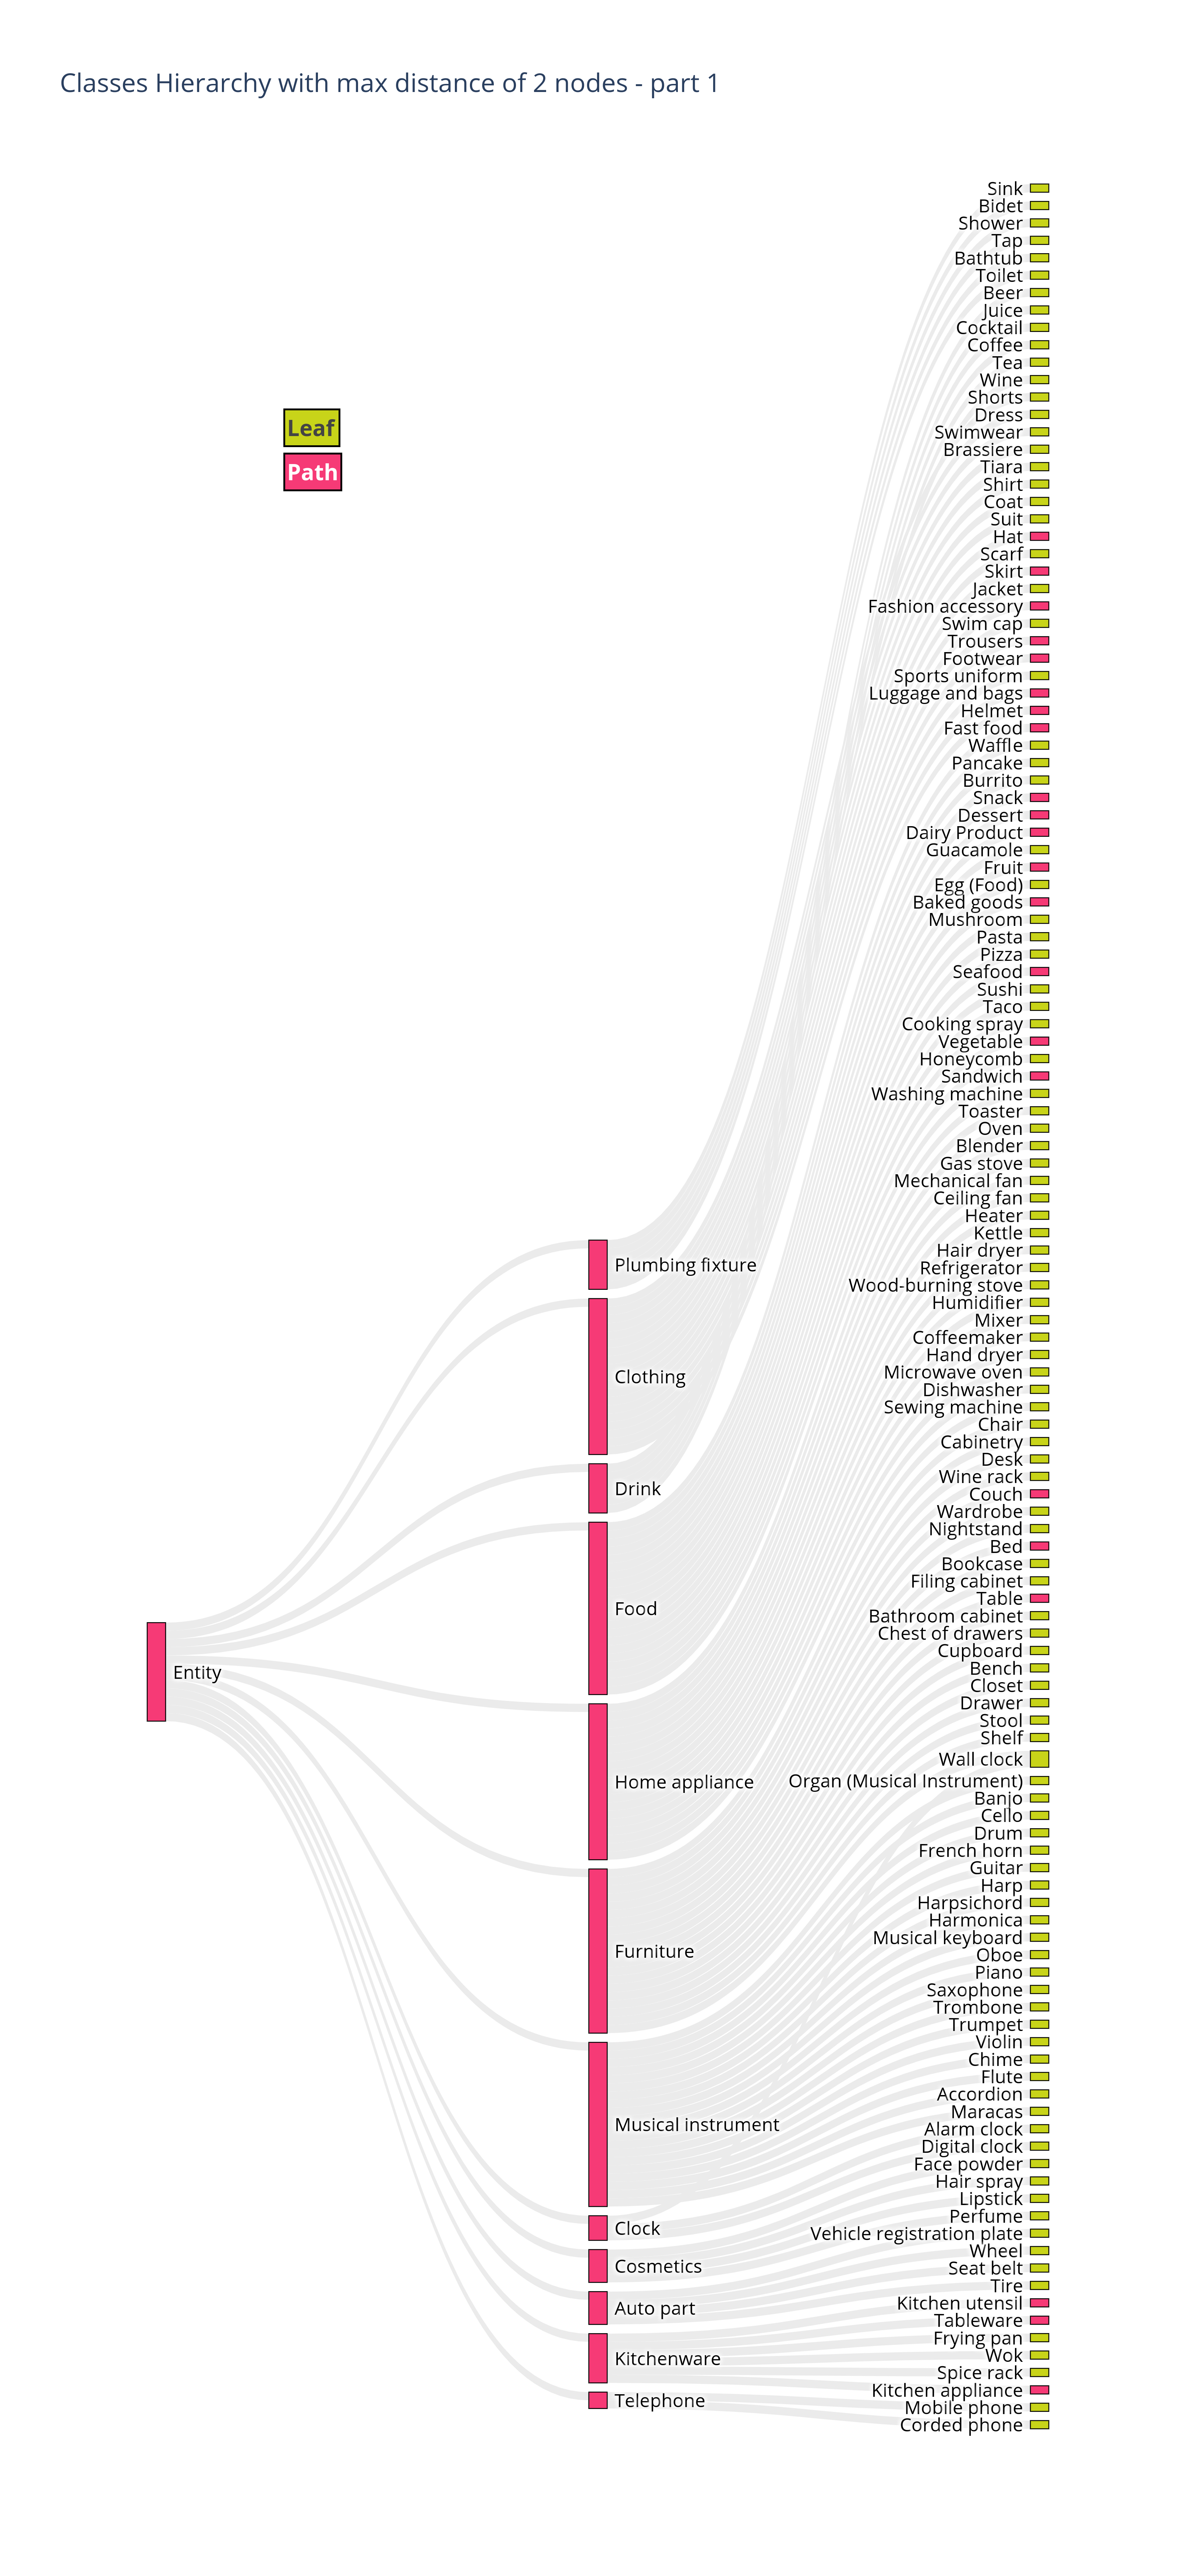
\includegraphics[width=0.7\textwidth]{lvl2_classes_pt1.png}
		\caption{\scriptsize Class Hierarchy - Second Level first part}
	\end{figure}
	\begin{figure*}[!ht]
		\centering
		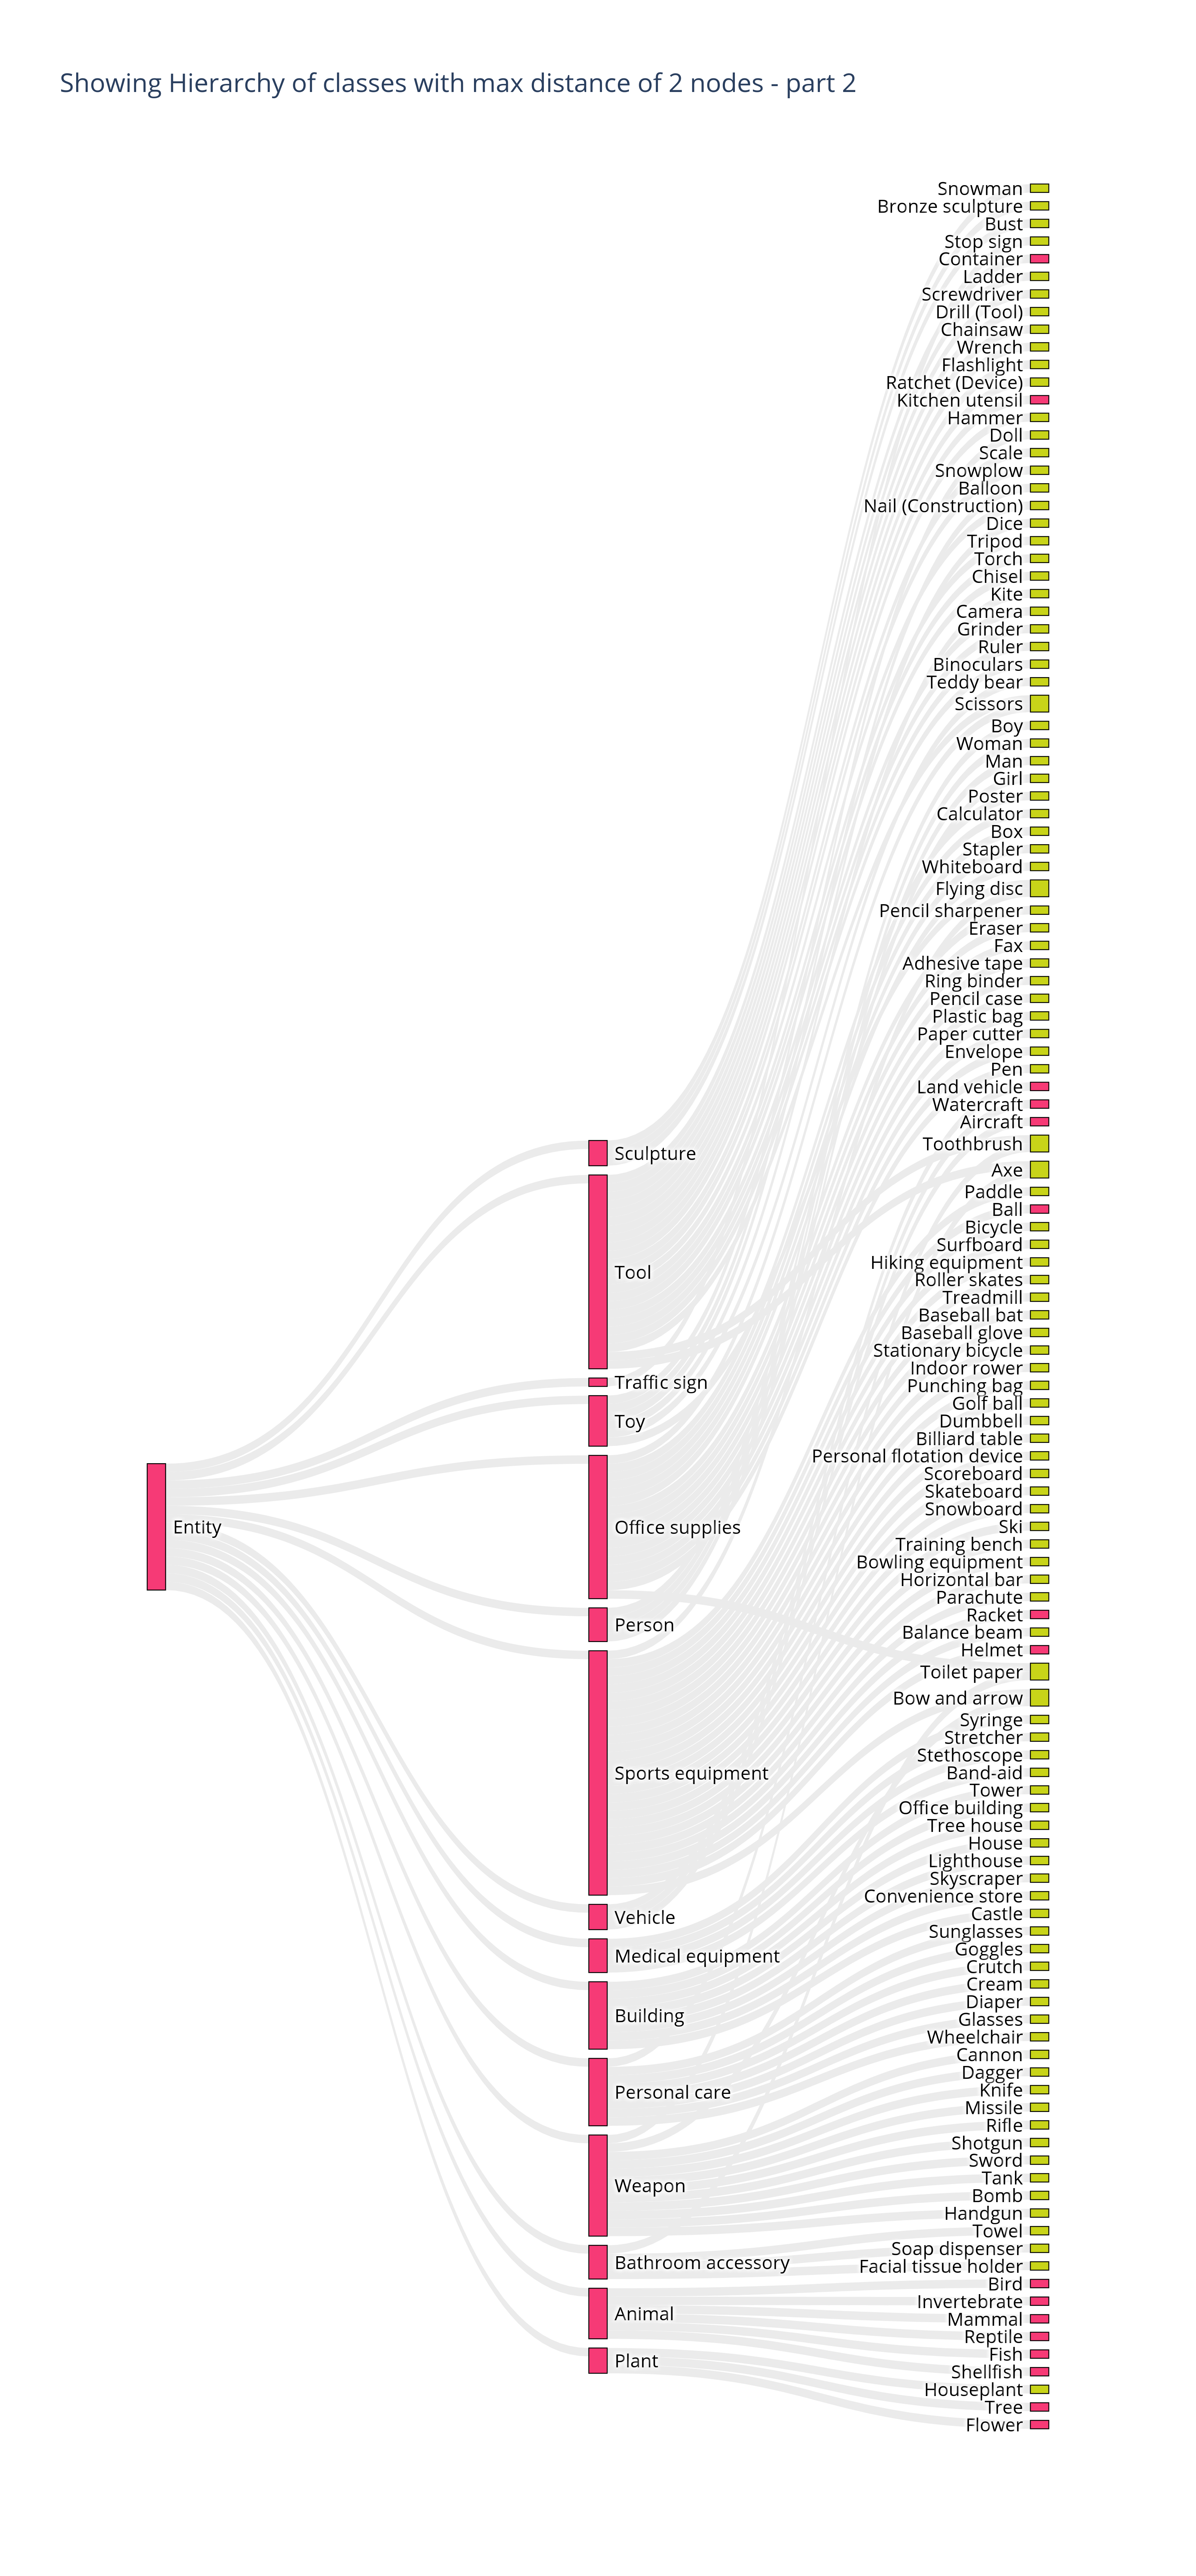
\includegraphics[width=0.7\textwidth]{lvl2_classes_pt2.png}
		\caption{\scriptsize Class Hierarchy - Second Level second part}
	\end{figure*}
	
	\begin{figure*}[!ht]
		\centering
		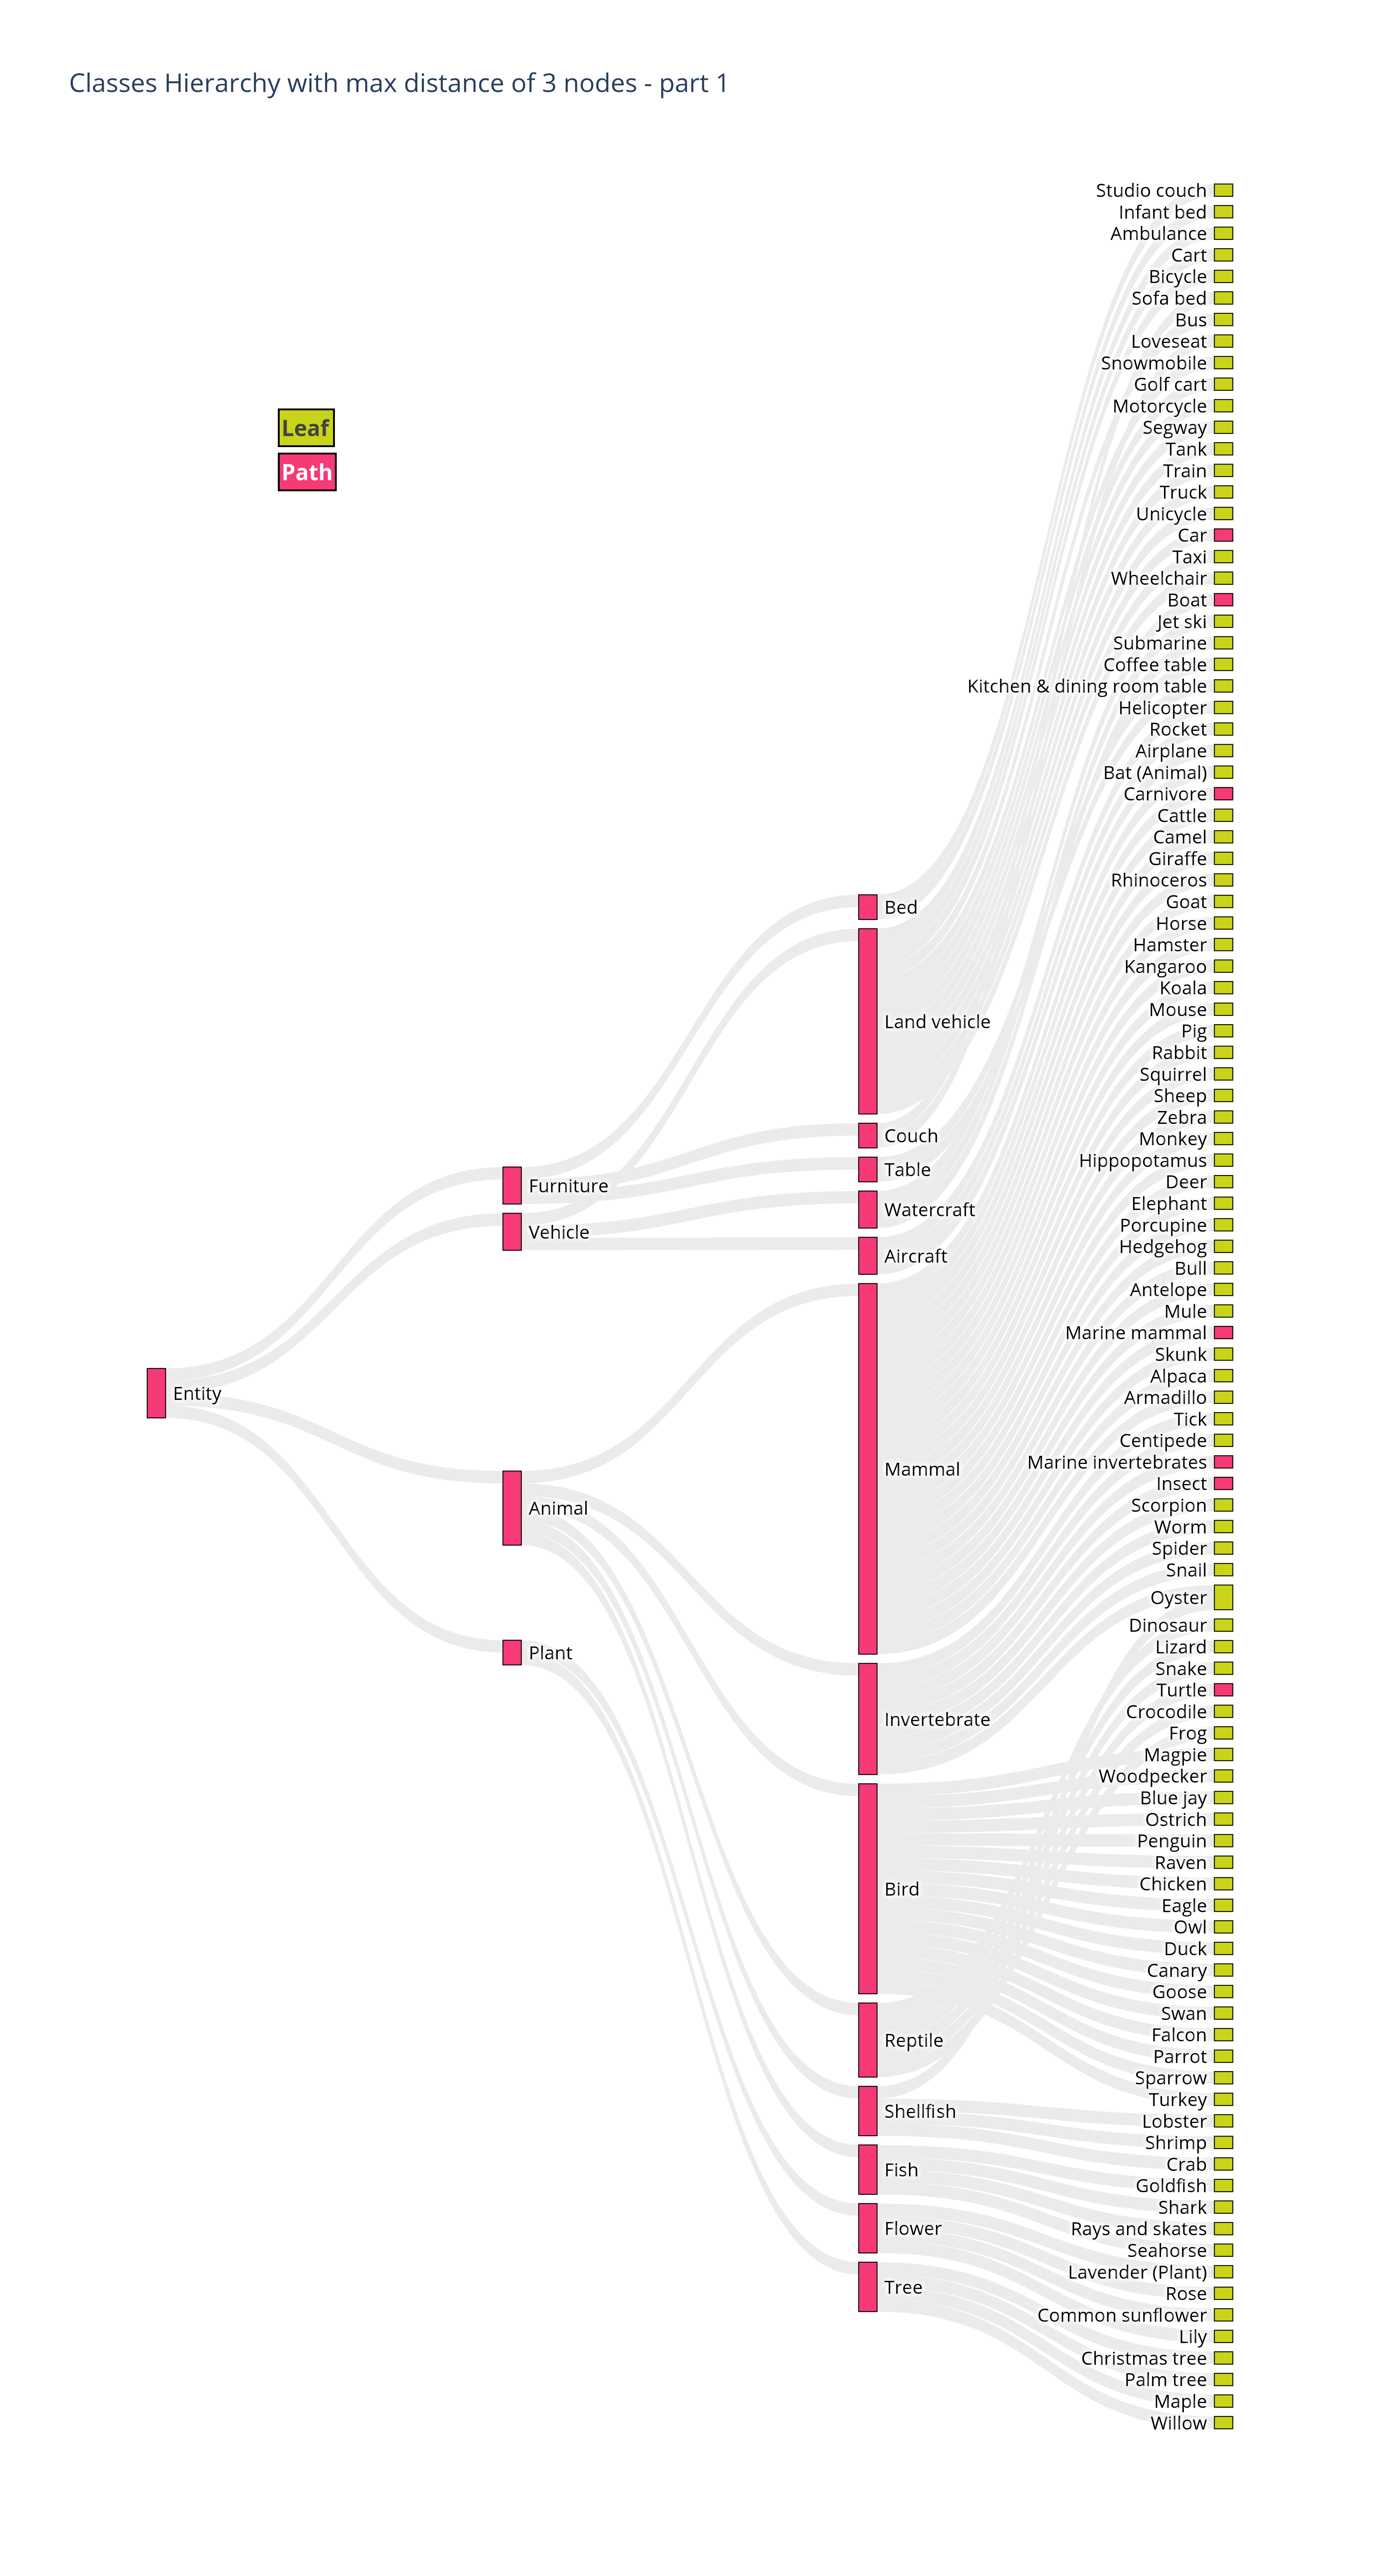
\includegraphics[width=0.8\textwidth]{lvl3_classes_pt1.png}
		\caption{\scriptsize Class Hierarchy - Third Level first part}
	\end{figure*}
	\begin{figure*}[!ht]
		\centering
		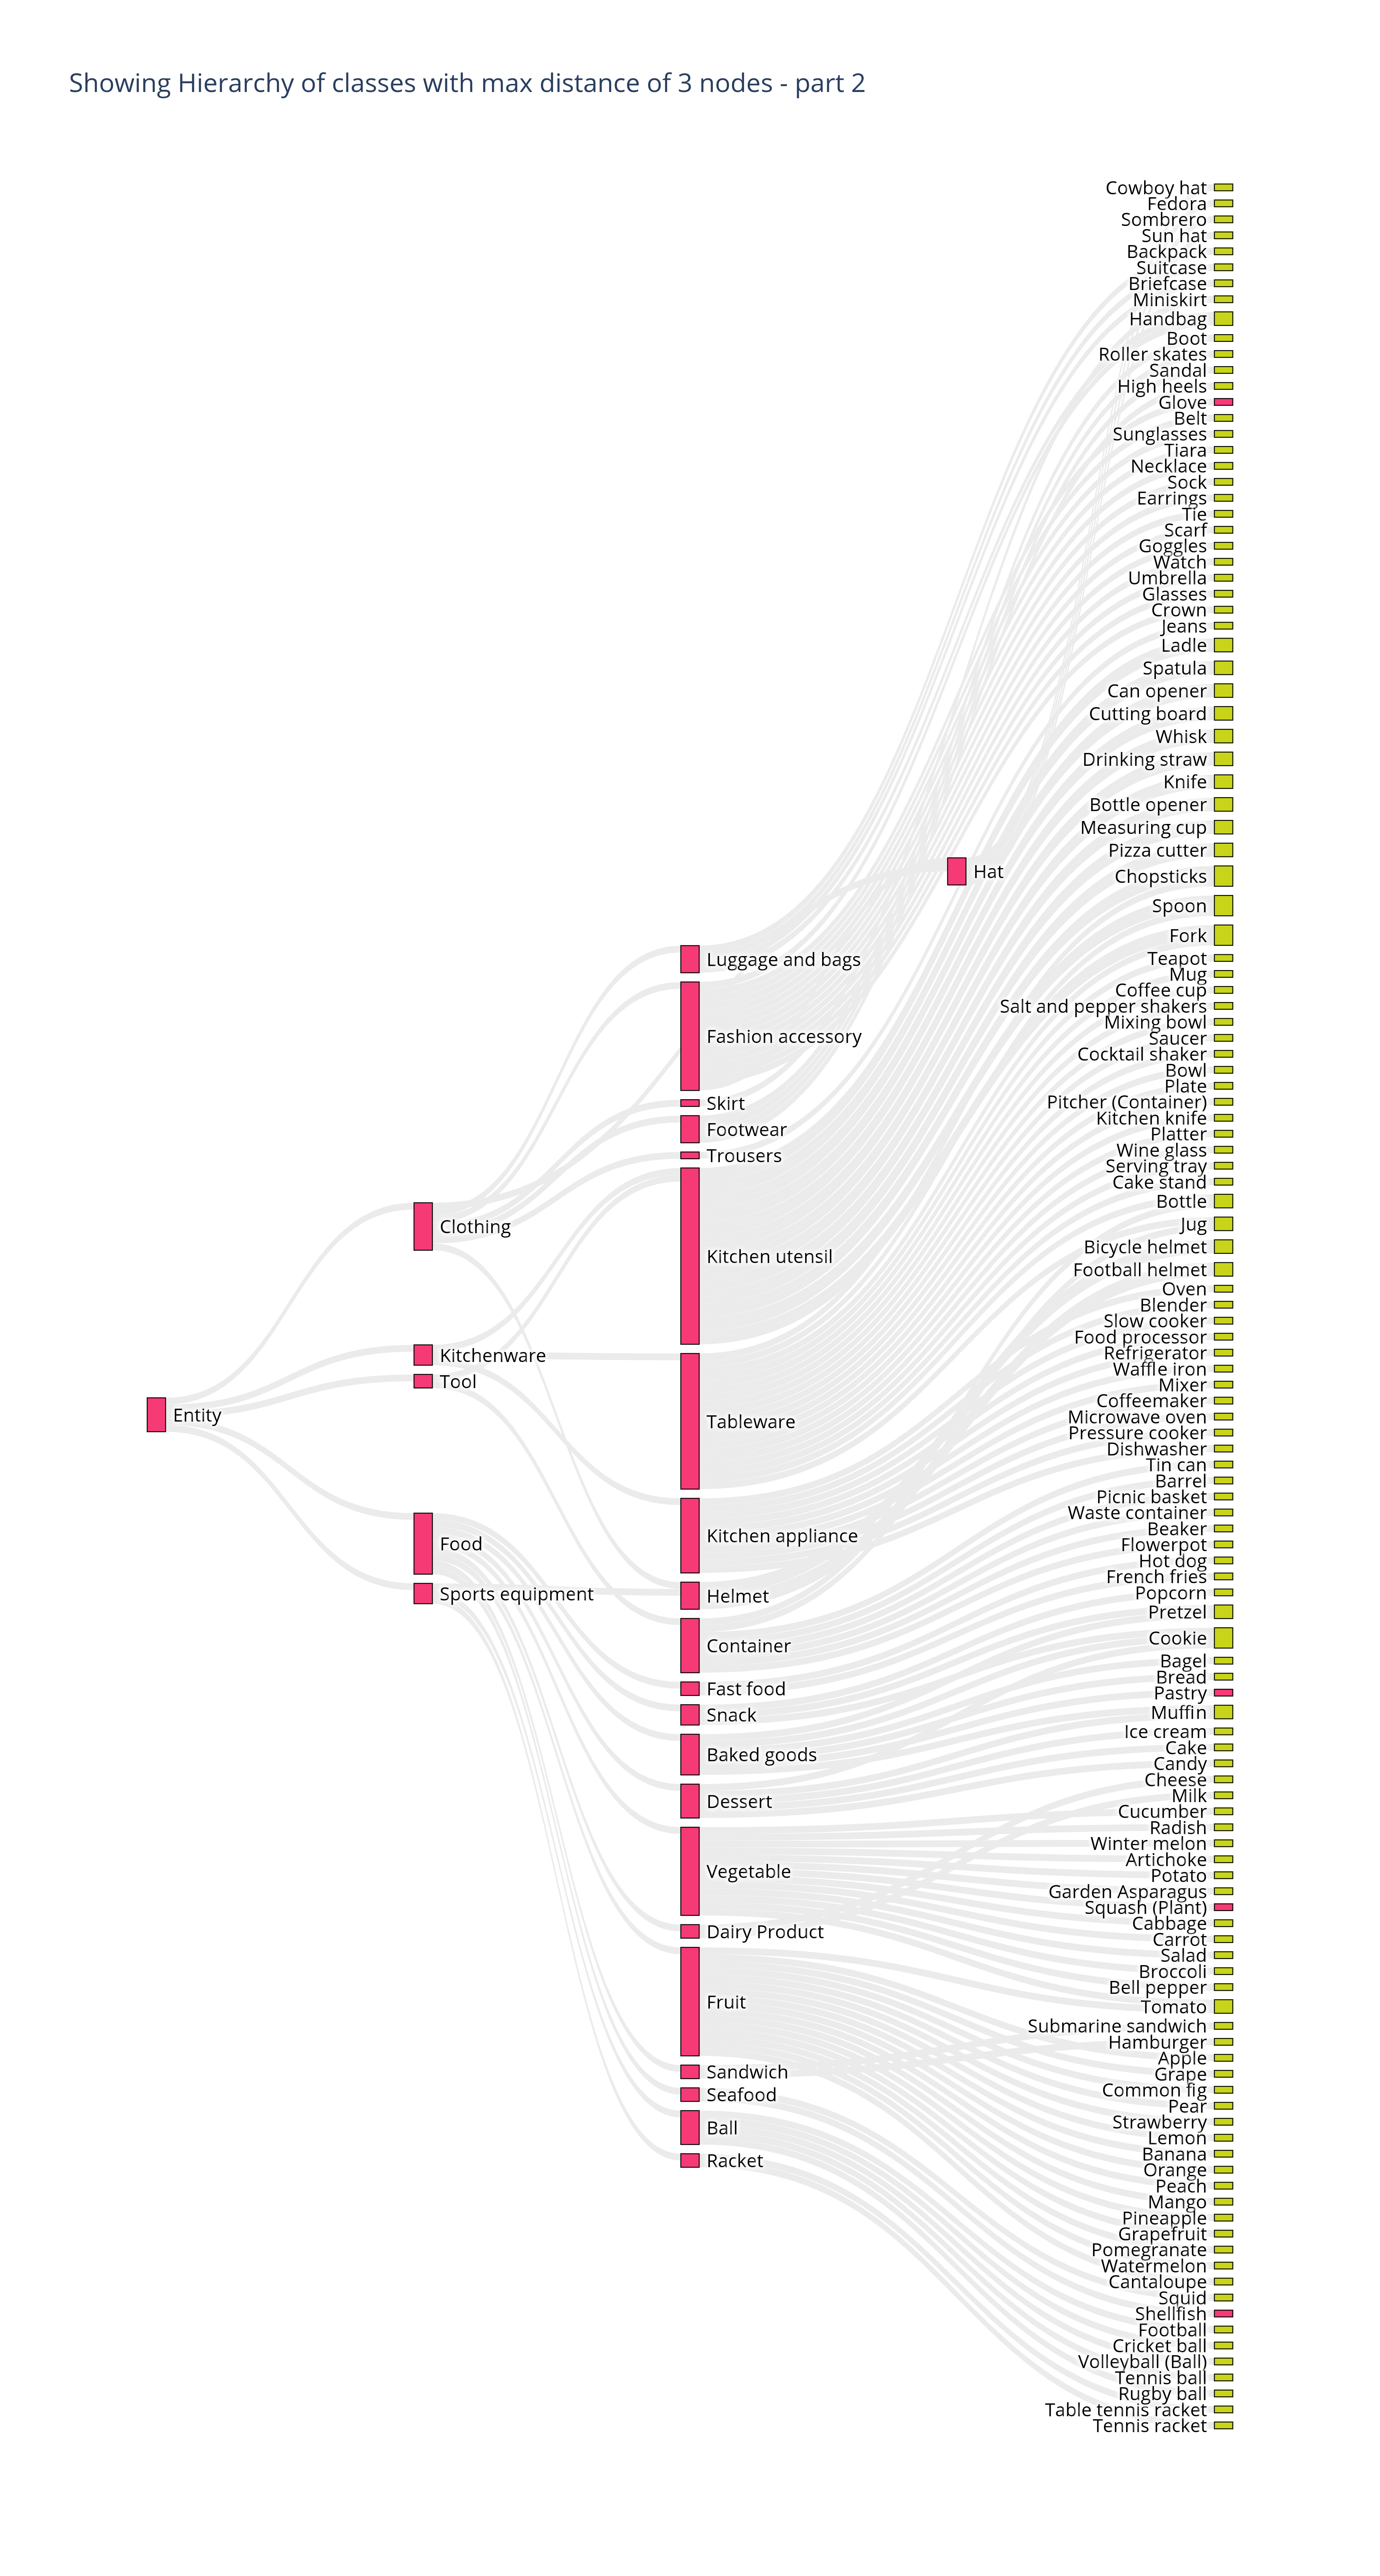
\includegraphics[width=0.8\textwidth]{lvl3_classes_pt2.png}
		\caption{\scriptsize Class Hierarchy - Third Level second part}
	\end{figure*}
	
	\begin{figure*}[!ht]
		\centering
		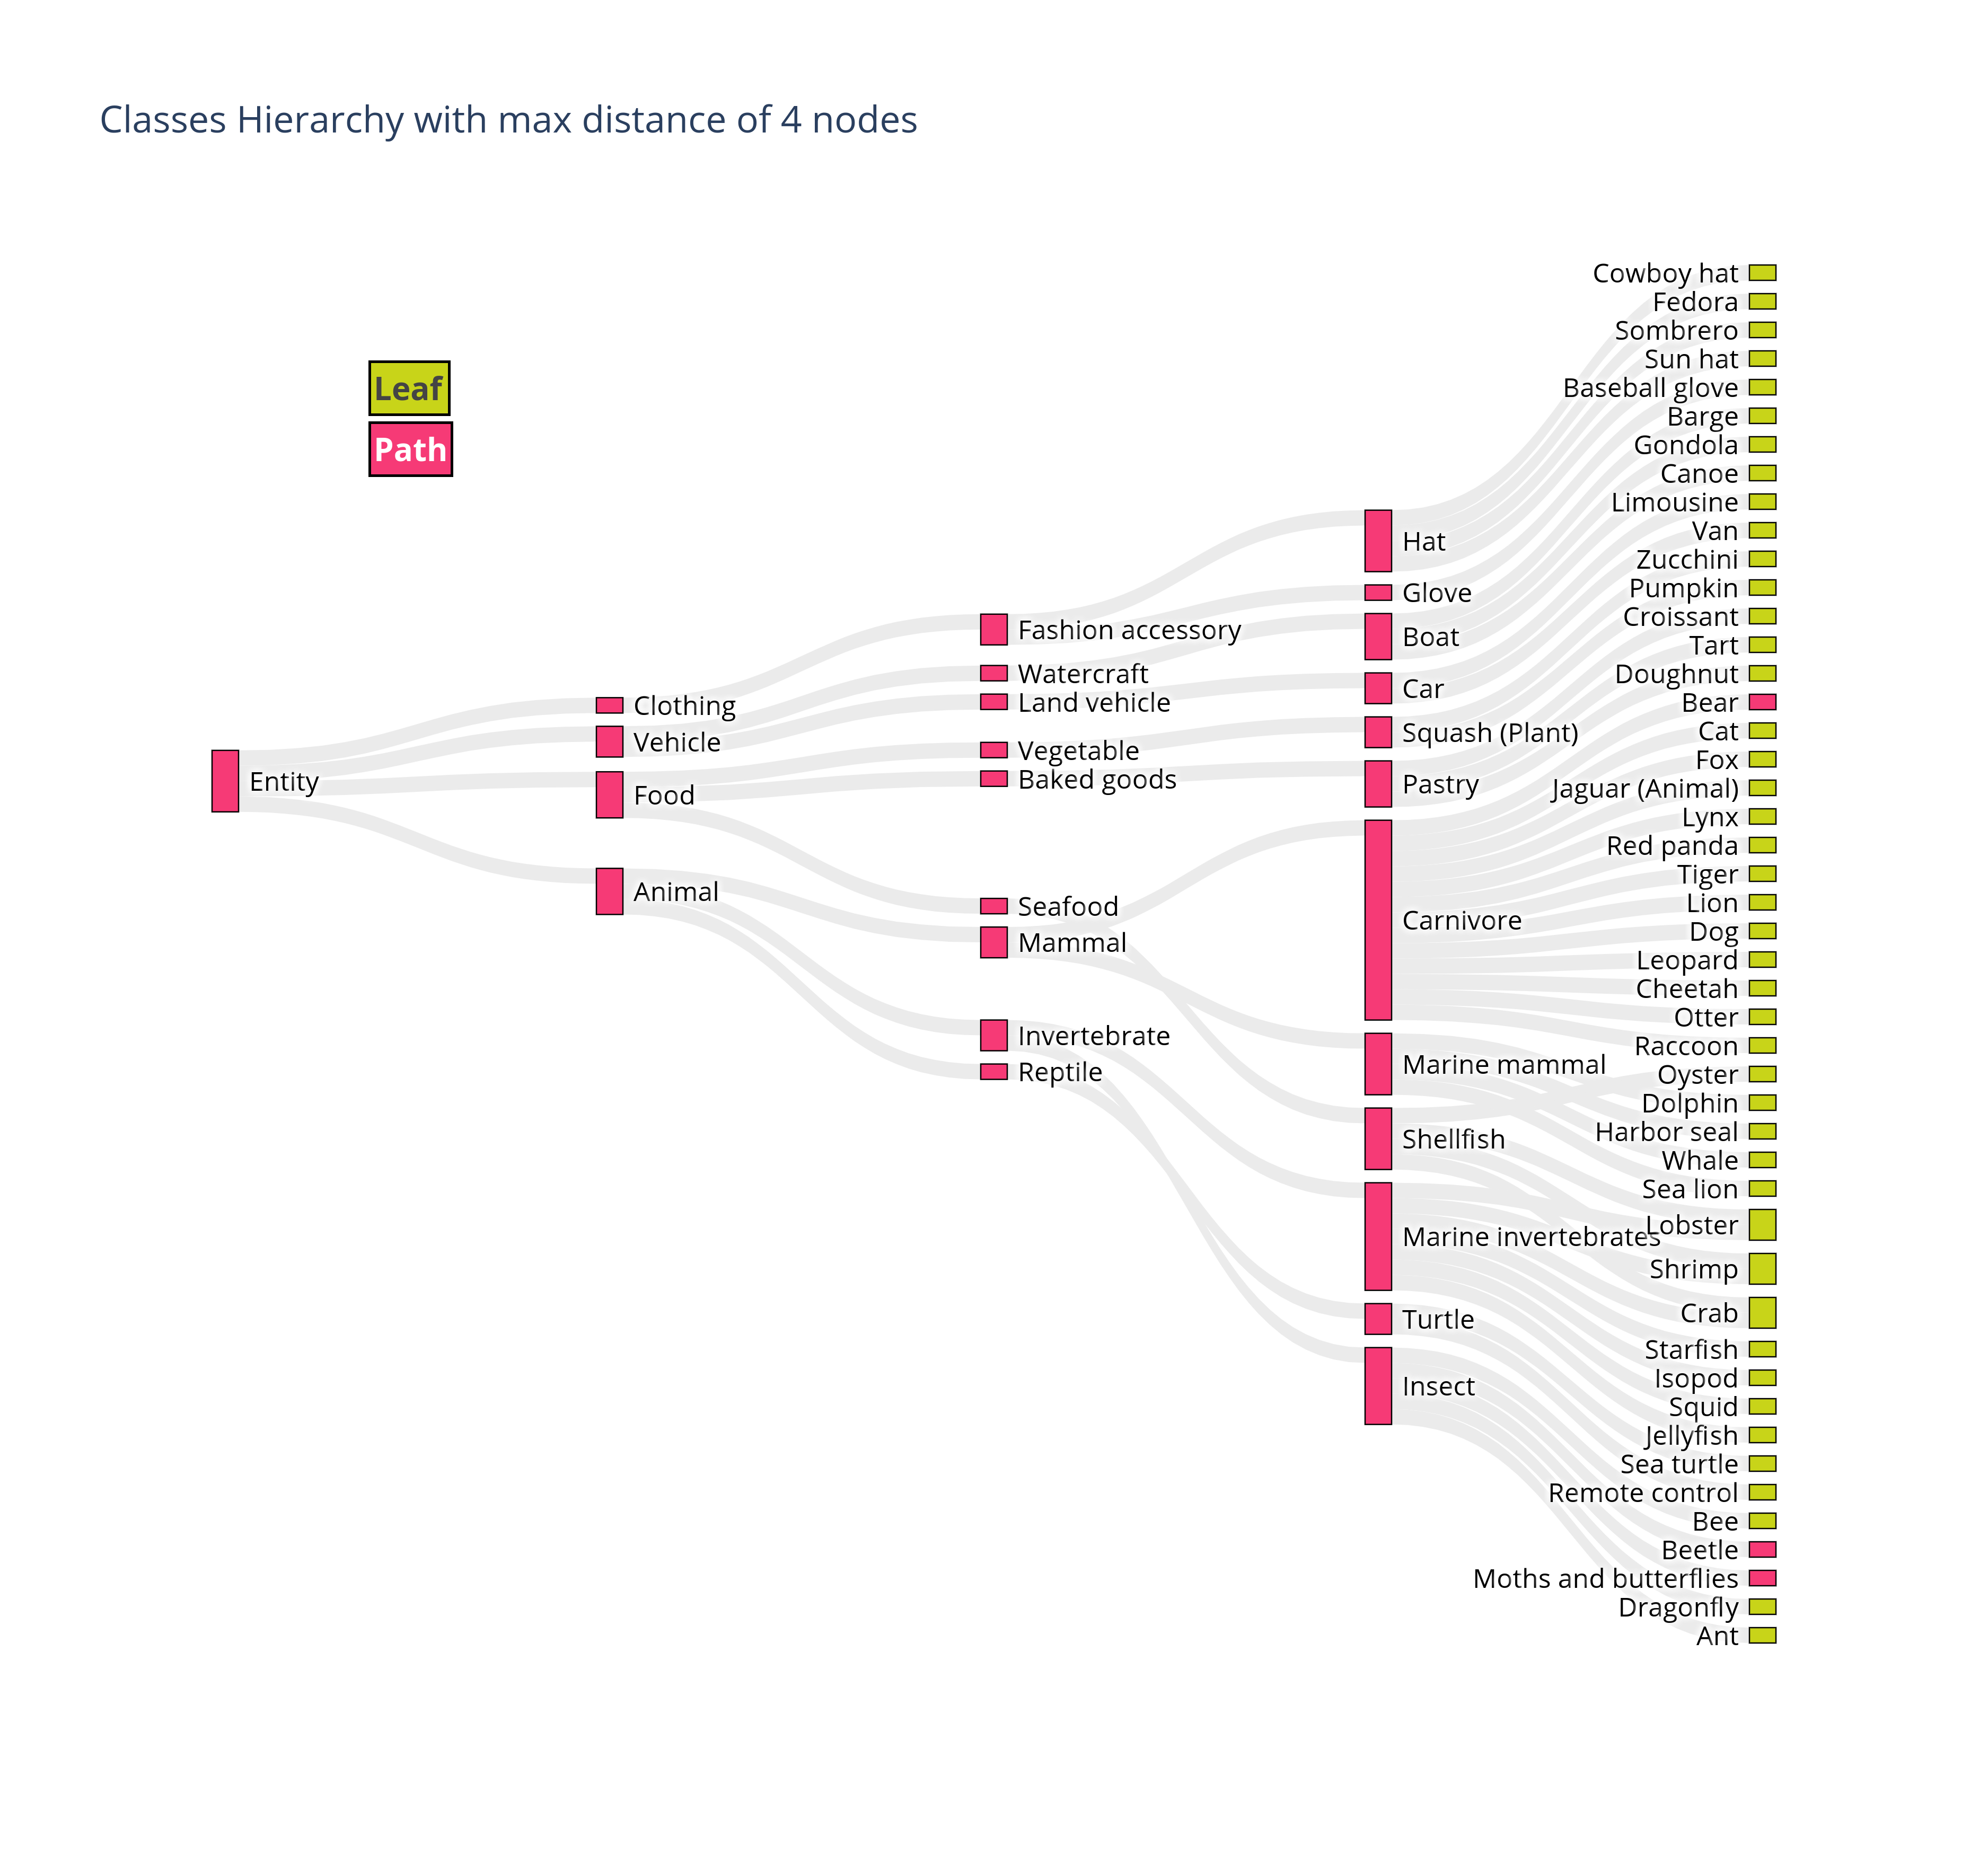
\includegraphics[width=0.8\textwidth]{lvl4_classes.png}
		\caption{\scriptsize Class Hierarchy - Fourth Level}
	\end{figure*}
	
	\begin{figure*}[!ht]
		\centering
		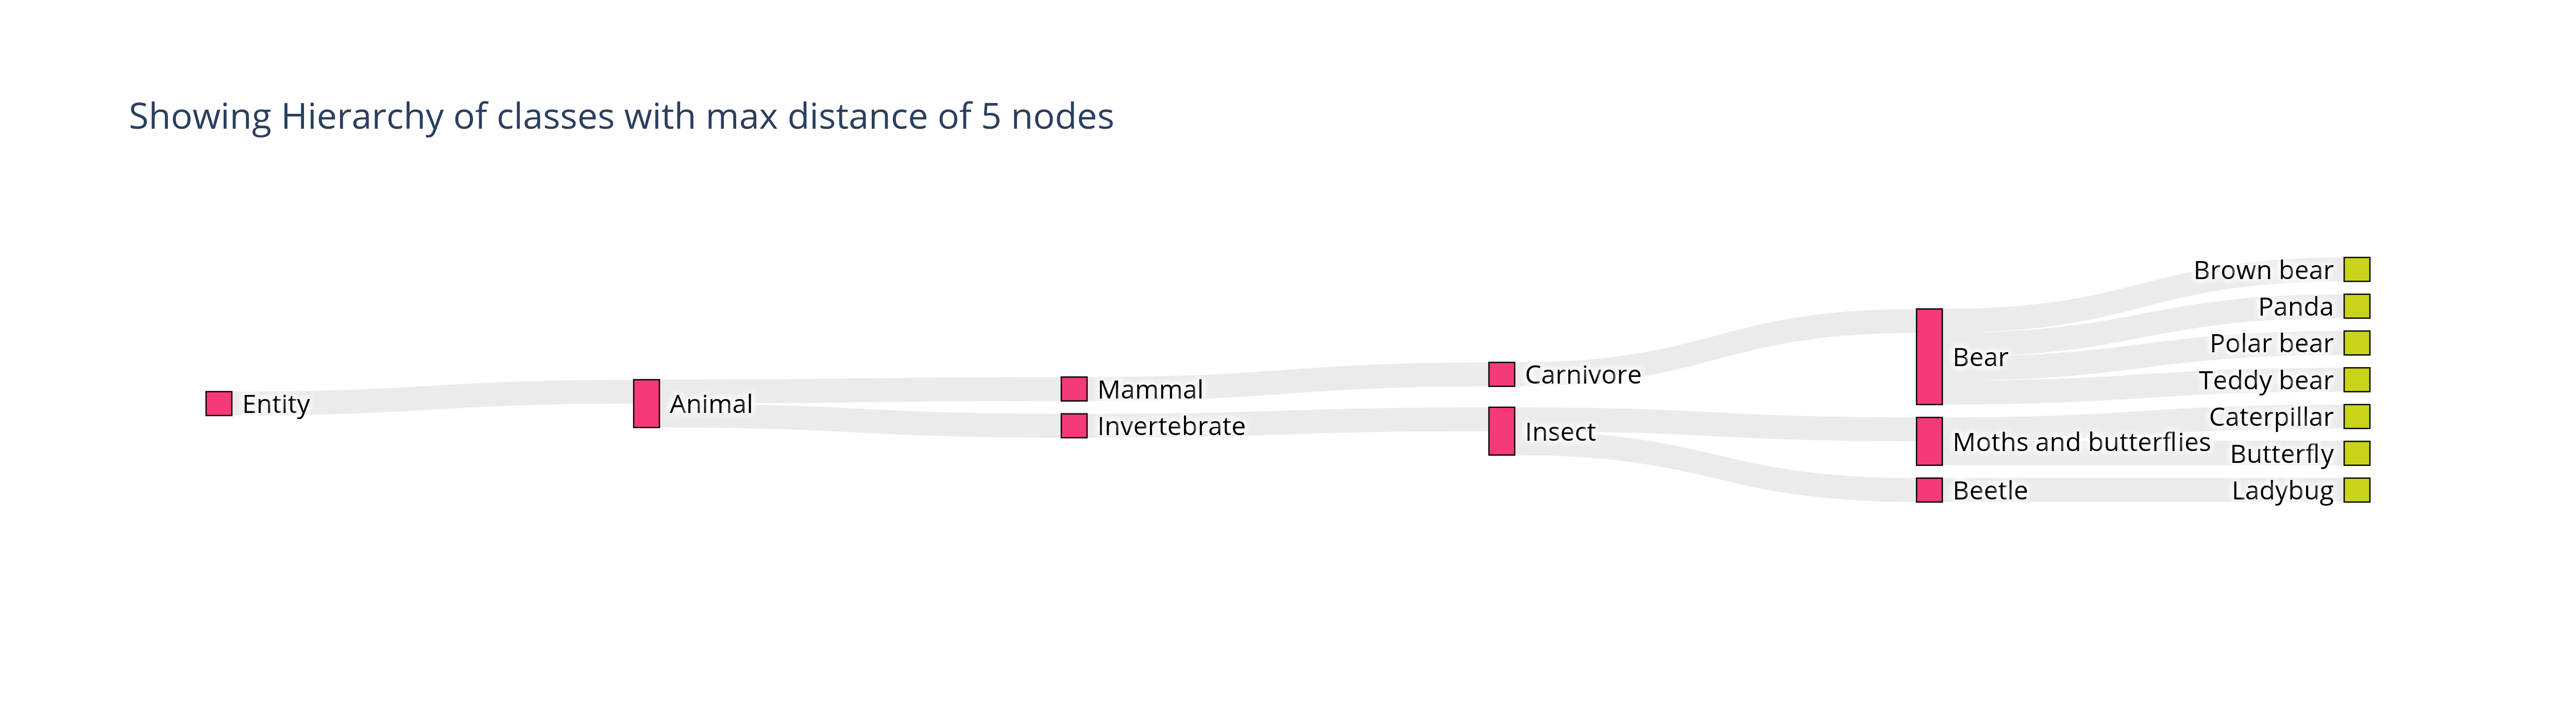
\includegraphics[width=0.8\textwidth]{lvl5_classes.png}
		\caption{\scriptsize Class Hierarchy - Fifth Level}
	\end{figure*}

\end{appendices}

\end{document}